%% Copernicus Publications Manuscript Preparation Template for LaTeX Submissions
%DIF LATEXDIFF DIFFERENCE FILE
%DIF DEL ./revision_1/LaTeX/manuscript.tex   Mon Jun 15 16:01:22 2026
%DIF ADD ./revision_2/LaTeX/manuscript.tex   Mon Jul 13 08:33:36 2026
%% ---------------------------------
%% This template should be used for copernicus.cls
%% The class file and some style files are bundled in the Copernicus Latex Package, which can be downloaded from the different journal webpages.
%% For further assistance please contact Copernicus Publications at: production@copernicus.org
%% https://publications.copernicus.org/for_authors/manuscript_preparation.html


%% Please use the following documentclass and journal abbreviations for preprints and final revised papers.

%% 2-column papers and preprints
\documentclass[hess, manuscript]{copernicus}
%\documentclass[hess]{copernicus}
\usepackage[compatibility=false]{caption}

%% Journal abbreviations (please use the same for preprints and final revised papers)
% Hydrology and Earth System Sciences (hess)


%% \usepackage commands included in the copernicus.cls:
%\usepackage[german, english]{babel}
\usepackage{tabularx}
%\usepackage{cancel}
%\usepackage{multirow}
%\usepackage{supertabular}
%\usepackage{algorithmic}
%\usepackage{algorithm}
%\usepackage{amsthm}
%\usepackage{float}
%\usepackage{subfig}
%\usepackage{rotating}
\usepackage{booktabs}
\usepackage{microtype}
\usepackage{threeparttable}

\newcommand{\calV}{OBJ-V}
\newcommand{\calQ}{OBJ-Q}
\newcommand{\calQV}{OBJ-QV}
\newcommand{\calGWW}{OBJ-V-GWW}
\newcommand{\KGEmod}{$\text{KGE}'$}
%DIF PREAMBLE EXTENSION ADDED BY LATEXDIFF
%DIF UNDERLINE PREAMBLE %DIF PREAMBLE
\RequirePackage[normalem]{ulem} %DIF PREAMBLE
\RequirePackage{color}\definecolor{RED}{rgb}{1,0,0}\definecolor{BLUE}{rgb}{0,0,1} %DIF PREAMBLE
\providecommand{\DIFadd}[1]{{\protect\color{blue}\uwave{#1}}} %DIF PREAMBLE
\providecommand{\DIFdel}[1]{{\protect\color{red}\sout{#1}}}                      %DIF PREAMBLE
%DIF SAFE PREAMBLE %DIF PREAMBLE
\providecommand{\DIFaddbegin}{} %DIF PREAMBLE
\providecommand{\DIFaddend}{} %DIF PREAMBLE
\providecommand{\DIFdelbegin}{} %DIF PREAMBLE
\providecommand{\DIFdelend}{} %DIF PREAMBLE
\providecommand{\DIFmodbegin}{} %DIF PREAMBLE
\providecommand{\DIFmodend}{} %DIF PREAMBLE
%DIF FLOATSAFE PREAMBLE %DIF PREAMBLE
\providecommand{\DIFaddFL}[1]{\DIFadd{#1}} %DIF PREAMBLE
\providecommand{\DIFdelFL}[1]{\DIFdel{#1}} %DIF PREAMBLE
\providecommand{\DIFaddbeginFL}{} %DIF PREAMBLE
\providecommand{\DIFaddendFL}{} %DIF PREAMBLE
\providecommand{\DIFdelbeginFL}{} %DIF PREAMBLE
\providecommand{\DIFdelendFL}{} %DIF PREAMBLE
%DIF COLORLISTINGS PREAMBLE %DIF PREAMBLE
\RequirePackage{listings} %DIF PREAMBLE
\RequirePackage{color} %DIF PREAMBLE
\lstdefinelanguage{DIFcode}{ %DIF PREAMBLE
%DIF DIFCODE_UNDERLINE %DIF PREAMBLE
  moredelim=[il][\color{red}\sout]{\%DIF\ <\ }, %DIF PREAMBLE
  moredelim=[il][\color{blue}\uwave]{\%DIF\ >\ } %DIF PREAMBLE
} %DIF PREAMBLE
\lstdefinestyle{DIFverbatimstyle}{ %DIF PREAMBLE
	language=DIFcode, %DIF PREAMBLE
	basicstyle=\ttfamily, %DIF PREAMBLE
	columns=fullflexible, %DIF PREAMBLE
	keepspaces=true %DIF PREAMBLE
} %DIF PREAMBLE
\lstnewenvironment{DIFverbatim}{\lstset{style=DIFverbatimstyle}}{} %DIF PREAMBLE
\lstnewenvironment{DIFverbatim*}{\lstset{style=DIFverbatimstyle,showspaces=true}}{} %DIF PREAMBLE
%DIF END PREAMBLE EXTENSION ADDED BY LATEXDIFF

\begin{document}

\title{Benchmarking reservoir operation schemes for large-scale hydrological models}

\Author[1,a][j.casado@kajoservices.com]{Jesús}{Casado-Rodríguez} %% correspondence author
\Author[2]{Juliana}{Disperati}
\Author[1]{Stefania}{Grimaldi}
\Author[1][peter.salamon@eu.europa.eu]{Peter}{Salamon}

\affil[1]{European Commission -- Joint Research Centre, Ispra, Italy}
\affil[2]{Fincons Group, Vimercate, Italy}
\affil[a]{now at: Kajo s.r.o., Banská Bystrica, Slovakia}
%\authorworkingcomment{Currently at Kajo s.r.o., Banská Bystrica, Slovakia}
%\authorcomment{Currently at Kajo s.r.o., Banská Bystrica, Slovakia}

\runningtitle{Benchmarking reservoir models in LSHM}
\runningauthor{Casado-Rodríguez et al.}

\received{}
\pubdiscuss{} %% only important for two-stage journals
\revised{}
\accepted{}
\published{}

%% These dates will be inserted by Copernicus Publications during the typesetting process.

\firstpage{1}

\maketitle



\begin{abstract}
There are approximately 62,000 large dams worldwide that significantly alter the hydrological regimes of most major rivers. Despite their importance, reservoirs remain poorly represented in Large-Scale Hydrological Models (LSHMs) due to the complexity of human-driven operations and a widespread lack of observational records. Consequently, reservoir routines in LSHMs must balance structural simplicity with limited data requirements. In this study, we utilize the ResOpsUS dataset to benchmark four reservoir routines of increasing complexity: LISFLOOD, CaMa-Flood, mHM, and STARFIT. We evaluate these routines across 164 reservoirs in the United States and test which target variables are most informative for parameter estimation. Our results indicate that the mHM routine consistently achieves the highest performance; however, its dependence on site-specific demand data limits its applicability at the global scale. In contrast, the CaMa-Flood routine provides a robust compromise, significantly outperforming the linear logic of LISFLOOD and matching the performance of the more complex STARFIT routine. This suggests that increased model complexity does not always yield superior results. Crucially, we find that calibrating to reservoir storage is more informative than calibrating to outflow, as it effectively captures the dynamics of both state variables. This finding paves the way for the use of satellite-derived storage products in the calibration of LSHMs. The findings of this study have been implemented in the upcoming versions of the European and Global Flood Awareness Systems (EFAS v6 and GloFAS v5).
\end{abstract}


%\copyrightstatement{TEXT} %% This section is optional and can be used for copyright transfers.


\introduction 

% Reservoir impacts: number and capacity, alteration of the water cycle, difficulties in forecasting discharge
%\citep{Wisser2010, Biemans2011, Scherer2016, Salwey2023, Moreno-Rodenas2025, Mulligan2020, Wang2022, ICOLD2024, Doll2009, Zhou2016}

The increasing global population and expanding economic activities have amplified the pressure on freshwater resources, making human interventions—such as the construction and operation of dams and reservoirs—fundamental elements of the terrestrial water cycle \citep{Biemans2011, Busker2019, Sadki2023, Moreno-Rodenas2025}. These structures are pivotal in fulfilling diverse societal needs, including domestic and industrial water supply, irrigation, hydropower production, and flood control \citep{Mekonnen2012, Abeshu2023, Sadki2023, Lehner2024, Shrestha2024, Moreno-Rodenas2025}. The global proliferation of dams has been unprecedented over the last century \citep{Lehner2024, Moreno-Rodenas2025}. Globally, there are approximately 62,000 large dams (heights > 15 m), cataloged by the ICOLD (International Commission on Large Dams)  \citep{Moreno-Rodenas2025}, with an estimated cumulative storage capacity ranging between 7,420 $\text{km}^3$  (GDW v1.0) \citep{Lehner2024} and 8,300 $\text{km}^3$ \citep{Sadki2023}. This volume represents roughly 20\% of the average annual river discharge to the oceans and is four times the amount of water stored in river channels worldwide \citep{Sadki2023}.

The immense scale of this intervention profoundly impacts natural hydrology by modifying the magnitude, timing, and duration of streamflows \citep{Shin2019, Salwey2024}, resulting in the fragmentation of over 60\% of the world's largest rivers \citep{Sadki2023}. In the contiguous United States (CONUS), dams regulate all major rivers, providing a total storage capacity equivalent to roughly 75\% of the mean annual CONUS runoff \citep{Steyaert2022}. While beneficial for human use, these operations cause significant environmental trade-offs, including the homogenization of river dynamics \citep{Scherer2016, Lehner2024}, alteration of sediment and nutrient transport \citep{Shin2019, Yassin2019}, and increased open-water evaporation, which can exacerbate water scarcity \citep{Scherer2016, Yassin2019, Liu2026}.

% Different model perspectives
Despite their importance, the accurate representation of complex reservoir operations remains a challenge in large-scale hydrological models (LSHMs) and land-surface models \citep{Turner2021, Sadki2023, Salwey2024}. Reservoir operations are intrinsically non-linear and governed by complex, human-driven decisions related to water demand, flood risk, and environmental constraints \citep{Coerver2018, Hanazaki2022, Steyaert2022, Salwey2024, Shrestha2024}. Consequently, models lacking adequate reservoir schemes often exhibit degraded predictive performance, especially in highly regulated basins \citep{Turner2021, Salwey2024, Steyaert2025}. Historically, global models have relied on generic operational rules utilizing static characteristics (e.g., capacity, primary purpose) from datasets like the Global Reservoir and Dam (GRanD) database \citep{Lehner2011}. However, these generic approaches often fail to capture the local operating behaviors necessary for simulating realistic daily releases and storage dynamics \citep{Turner2021}. Recent research has therefore pivoted toward exploiting newly available observational data and integrating data-driven techniques, such as machine learning or statistically inferred policies, to better reflect historical decision-making \citep{Coerver2018, Turner2021, Steyaert2025}.

% Introduction to GloFAS and the need for  better reservoir representation
This research aims to improve the reservoir module within the OS LISFLOOD hydrological model \citep{DeRoo2000, vanderKnijff2010, Burek2013a, JRC2026}, a core component of the Global and European Flood Awareness Systems of the Copernicus Emergency Management Services (GloFAS and EFAS) \citep{EFAS2026, GloFAS2026}. The current LISFLOOD reservoir module employs an operation scheme based on three fixed storage limits (conservation, normal, and flood pools) without explicit classification of reservoir purpose  \citep{Zajac2017}. Our objective is to identify a reservoir routine suitable for global application—one that balances portability with efficacy in data-scarce environments.

Specifically, this study presents a systematic benchmark comparing the performance of four distinct reservoir schemes within large-scale hydrological models, all of which are calibrated using in-situ records. We selected schemes from the literature that represent an increasing level of complexity and varying modeling philosophies: the current LISFLOOD storage-based parameterization \citep{Zajac2017}, its evolution as implemented in CaMa-Flood \citep{Hanazaki2022}, a demand-driven approach from mHM \citep{Shrestha2024}, and a seasonality-driven statistical approach, STARFIT \citep{Turner2021}. While not exhaustive, this selection encompasses the primary modeling paradigms currently used in the field. Other models, such as DZTR \citep{Yassin2019} or SBTS \citep{Shen2025}, could be evaluated in future work. By assessing the capability of these schemes to simulate observed flow regulation and storage dynamics, this research provides critical guidance for the development of human–water interaction modules in the next generation of operational flood systems and LSHMs.

A novel aspect of this study is the exploration of a decoupled calibration strategy, where the reservoir routines are evaluated in isolation from the rest of the catchment hydrology. Rather than calibrating reservoir parameters simultaneously with the rest of the hydrological model against downstream river discharge—a process often plagued by equifinality \citep{Beven2001}—we model reservoir management as a standalone system. To achieve this, we selected reservoirs with observed inflow, outflow, and storage records. This approach ensures that reservoir parameters are sensitive to actual operations rather than compensating for upstream hydrological biases or being masked by gauge observations far downstream.

However, the practical implementation of this strategy faces a significant data bottleneck. While in situ records of reservoir outflow provide the most direct target for calibration, such data are frequently inaccessible or classified as proprietary. Consequently, river discharge measured at gauging stations downstream of the reservoir is often used as a proxy for reservoir operations. This approach inherently assumes that total reservoir outflow is equivalent to river discharge—an assumption that fails when significant volumes are diverted for hydropower, irrigation, or municipal supply. To overcome these limitations, satellite-derived products offer a promising alternative \citep{Schwatke2015, Pekel2016, Schwatke2020, Donchyts2022, Khandelwal2022, Hao2024, Hou2024}. These products offer the potential to monitor volume fluctuations in ungauged regions, making them crucial for future global model calibration and data assimilation \citep{Hanazaki2022, Shen2025, Steyaert2025}.

A calibration based on satellite products would target reservoir level or storage, instead of outflow (or river discharge as a proxy variable). To assess the feasibility of using satellite products, we compare the performance of the model when calibrated against three distinct targets: (i) reservoir release only, (ii) reservoir storage only, and (iii) a combined objective function utilizing both variables. By evaluating these configurations, this study aims to assess whether satellite-inferred storage can serve as a robust alternative to ground-based outflow records, thereby enabling improved reservoir modeling in ungauged or data-scarce regions. 

% mention difficulties in accessing ground-based data
% \citep{Zhou2016}
The benchmarking is supported by the ResOpsUS dataset \citep{Steyaert2022, Steyaert2024}, the first comprehensive, national-scale inventory providing historical daily reservoir operations for 679 major dams across the CONUS. ResOpsUS includes records of reservoir inflow, level, storage and outflow (not all variables for all reservoirs), providing the necessary variables for our benchmark. We leverage this data-rich environment to test the models and calibration targets, establishing a proof-of-concept for operational environments where such granular data is unavailable.

In summary, this study benchmarks four reservoir modeling paradigms across the CONUS domain to address three primary objectives: (i) to identify the most robust reservoir routine for continental or global hydrological models; (ii) to determine the most suitable target variable for calibration—storage, outflow, or both; and (iii) to evaluate the feasibility of using remotely-sensed storage data in the calibration of large-scale models.



\section{Data}
\label{sec:data}

\subsection{Reservoir Selection and Filtering}
\label{sec:reservoir_selection}

To evaluate reservoir routines in a data-rich context, we utilized the ResOpsUS dataset \citep{Steyaert2022, Steyaert2024}, which provides daily time series of reservoir operations for 679 reservoirs across the CONUS. From this initial pool, we applied a rigorous filtering process to ensure the suitability of the reservoirs for LSHM:

\begin{enumerate}
    \item Data Availability: We selected only those reservoirs containing concurrent daily records for all three primary variables: inflow ($I$), storage ($V$), and outflow ($Q$).
    \item Physical Dimensions: Reservoirs were required to have a minimum catchment area of 50~km² and a minimum storage capacity ($V_{\max}$) of 10~hm³.
    \item Hydrological Impact: Large-scale hydrological models such as GloFAS or EFAS are primarily focused on modelling river streamflow. For the sake of parsimony, we only want to include in those systems "disruptive" reservoirs—those that significantly alter the downstream flow regime. \citet{Shrestha2024} devised two thresholds that identify disruptive reservoirs using the Degree of Regulation ($\text{DOR}$; Eq.~\ref{eq:degree_of_regulation}) and the Degree of Disruptivity ($\text{DOD}$; Eq.~\ref{eq:degree_of_disruptivity}). Following their recommendations, only reservoirs with $\text{DOR} \geq 0.08$ and $\text{DOD} \geq 0.06$~m were selected:
    \begin{subequations}
        \label{eq:disruptive_reservoirs}
        \begin{align}
            \text{DOR} &= \frac{V_{\max}}{\bar{I}_{\text{yr}}} \quad [-] \label{eq:degree_of_regulation} \\[1ex]
            \text{DOD} &= \frac{V_{\max}}{A_c} \quad [\text{m}] \label{eq:degree_of_disruptivity}
        \end{align} 
    \end{subequations}
    where $V_{\max}$ is the reservoir storage capacity [m$^3$], $\bar{I}_{yr}$ is the average annual inflow [m$^3$/year], and $A_c$ is the catchment area [m$^2$].
    \item Record Length: To ensure sufficient data for robust model calibration, we removed reservoirs with time series shorter than four years.
    \item Water Balance Integrity: Preliminary analysis revealed large biases between average inflow and outflow in several reservoirs. Such discrepancies may stem from poor data quality or significant consumptive use (e.g., water diversions) not explicitly represented in our modeling framework. To ensure a closed water balance for benchmarking, we removed reservoirs where the absolute bias exceeded 30\%.
\end{enumerate}

Applying these criteria resulted in a final selection of 164 reservoirs. Their geographical distribution, categorized by catchment area and storage capacity, is depicted in Fig.~\ref{fig:map_reservoirs}.

\begin{figure*}
    \centering
    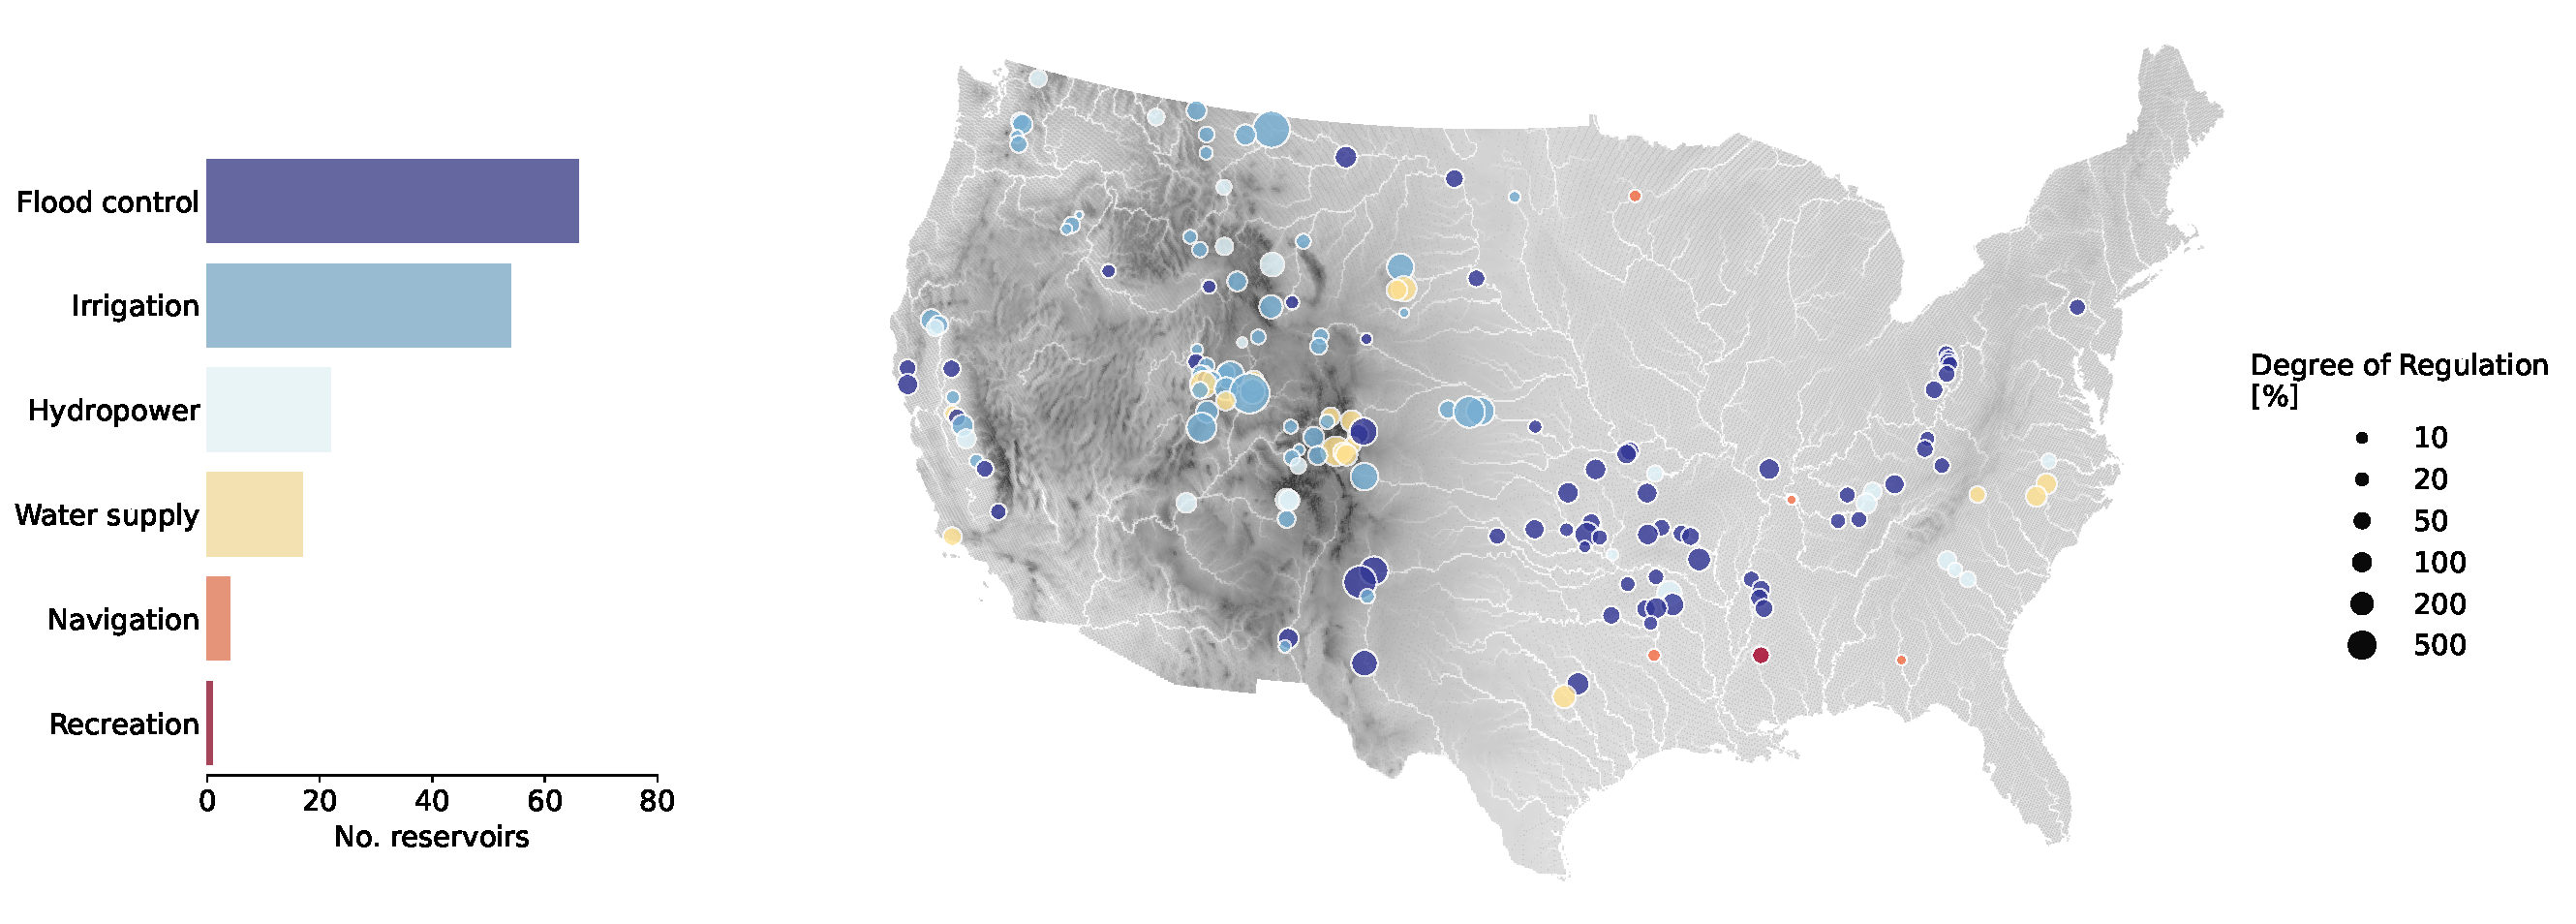
\includegraphics[width=\textwidth]{figures/fig01.pdf}
    \caption{Distribution of the 164 reservoirs from the ResOpsUS dataset used in the benchmarking. Colors represent the main reservoir use and point size the degree of regulation.}
    \label{fig:map_reservoirs}
\end{figure*}

\subsection{Dataset Integration and Attribute Enrichment}
\label{sec:reservoir_attributes}

To satisfy the input requirements of the diverse reservoir routines, we enriched the ResOpsUS records with supplementary hydrometeorological time series, and catchment and reservoir attributes.

As detailed in Sect.~\ref{sec:reservoir_models}, the routines require time series of direct precipitation and evaporation. These were extracted for each reservoir location from the ERA5 reanalysis dataset \citep{Hersbach2020}. 

Static reservoir and dam attributes were primarily sourced from the Global Reservoir and Dam dataset (GRanD) \citep{Lehner2011}. While we included all GRanD attributes in our dataset, four were critical for the simulations: storage capacity ($V_{\max}$), maximum surface area ($A_{\max}$), dam crest elevation ($Z_{\max}$), and dam height ($H_{\text{dam}}$). A comparison of these attributes against observed time series revealed inconsistencies in some attribute values. To rectify this, we cross-referenced GRanD with the Global Dam Watch (GDW) dataset \citep{Lehner2024}. For instances where the attributes remained inconsistent, we manually updated the records using official data from U.S. authorities, including the U.S. Army Corps of Engineers' National Inventory of Dams (NID), the U.S. Bureau of Reclamation (USBR), and the U.S. Geological Survey (USGS) \citep{NID, USBR, USGS}. Similar errors were reported by \citet{Shrestha2024}.

For the purpose of parameter regionalization or the development of data-driven models, we further included catchment-scale characteristics derived from GloFAS surface fields \citep{Choulga2024} and climate indices derived from ERA5 \citep{Hersbach2020}. 

We named the enriched dataset \textit{Reservoir Operations US and CAtchment and Reservoir Static attributes} (ResOpsUS+CARS). It is available via \href{https://doi.org/10.5281/zenodo.15978041}{Zenodo}. The dataset structure follows the standards defined by the CARAVAN initiative \citep{Kratzert2023}, ensuring it is formatted for immediate use in deep learning and large-sample hydrological studies.

The specific time series and static attributes from ResOpsUS+CARS utilized in this study are summarized in Table~\ref{tab:data}. These include model forcing inputs, variables for calibration and evaluation, and geometric parameters used for the estimation of reservoir area or elevation.

\begin{table}[t]
    \centering
    \caption{Data included in the ResOpsUS+CARS dataset used in this study.}
    \label{tab:data}
    \begin{tabular*}{\columnwidth}{@{\extracolsep{\fill}}lllll}
        \toprule
        \textbf{Category} & \textbf{Variable} & \textbf{Source} & \textbf{Units} & \textbf{Purpose} \\
        \midrule
        Time & Inflow & [1] & $\text{m}^3\,\text{s}^{-1}$ & Model input \\
        series & Storage & [1] & $10^6\,\text{m}^3$ & Calib./Eval. \\
        & Outflow & [1] & $\text{m}^3\,\text{s}^{-1}$ & Calib./Eval. \\
        & Elevation & [1] & m\,a.s.l. & Evaluation \\
        & Precipitation & [2] & mm & Model input \\
        & Evaporation & [2] & mm & Model input \\
        \midrule
        Attributes & Capacity & [3] & $10^6\,\text{m}^3$ & Model input \\
        & Surface Area & [3] & $\text{km}^2$ & Area estim. \\
        & Crest Elevation & [3] & m\,a.s.l. & Elev. estim. \\
        & Dam Height & [3] & m & Elev. estim. \\
        \bottomrule
    \end{tabular*}
    \small
    \smallskip
    \textit{Sources:} [1] ResOpsUS; [2] ERA5; [3] GRanD.
\end{table}

\section{Methods}
\label{sec:methods}

\subsection{Reservoir models}
\label{sec:reservoir_models}

Each of the reservoir routines evaluated in this study is governed by the water mass balance equation (Eq.~\ref{eq:mass_balance}). At each time step $\Delta t$, the model calculates the reservoir storage at the end of the interval ($V_{t+1}$) based on the preceding storage state ($V_t$), the water surface area ($A_t$), and three forcing variables: inflow ($I_t$), precipitation ($P_t$), and evaporation ($E_t$):

\begin{equation}
    \label{eq:mass_balance}
    V_{t+1} = V_t + \left( P_t - E_t \right) \cdot A_t + \left( I_t - Q_t \right) \cdot \Delta t 
\end{equation}

where $Q_t$ is the reservoir outflow (release), the fundamental difference between the four reservoir schemes. 

To represent the reservoir's bathymetry, we assume an inverted half-pyramid geometry (Fig.~\ref{fig:reservoir_scheme}), following the approach of \citet{Liebe2005} and subsequent studies \citep{Shin2019, Sadki2023, Shrestha2024}.This geometric approximation allows for the continuous estimation of the water surface area (Eq.~\ref{eq:area}), which is required for the mass balance, and the water level ($Z_t$; Eq.~\ref{eq:level}), provided that the dam crest elevation and the dam height are known. We evaluate the validity of this geometric assumption by comparing estimated levels against observed records in a subset of reservoirs where such data is available.

\begin{figure}
    \centering
    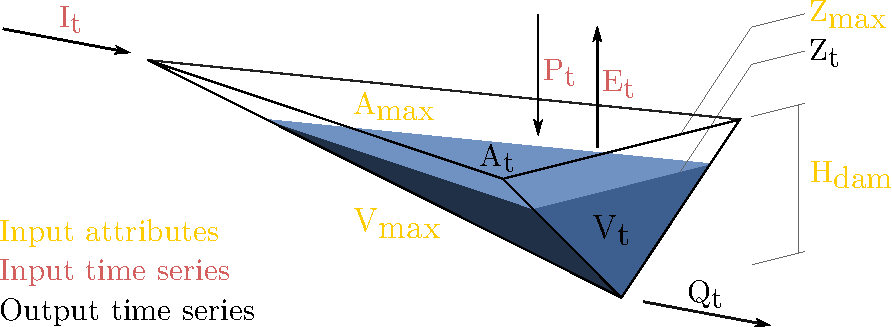
\includegraphics[width=\columnwidth]{figures/fig02.pdf}
    \caption{Simplified reservoir shape adopted in this study, including all the model input and output variables.}
    \label{fig:reservoir_scheme}
\end{figure}

\begin{subequations}
\label{eq:reservoir_geometry}
\begin{align}
    A_t &= A_{\max} \Bigl( \frac{V_t}{V_{\max}} \Bigr)^{2/3} \label{eq:area} \\[1ex]
    Z_t &= Z_{\max} - H_{\text{dam}} \left[ 1 - \Bigl( \frac{V_t}{V_{\max}} \Bigr)^{1/3} \right] \label{eq:level}
\end{align}
\end{subequations}

\subsubsection{LISFLOOD}
\label{sec:lisflood}

The current LISFLOOD reservoir routine \citep{Burek2013a, Zajac2017} operates as a piecewise linear storage-outflow relationship. The release is determined by the storage zone in which the reservoir resides at any given time step: conservative, normal or flood.

\begin{equation}
    \label{eq:lisflood}
    \begin{split}
    & Q_t = \\
    & \begin{cases}
        Q_c & \text{if } V_t < 2 V_c \\
        Q_c + ( Q_n - Q_c ) \frac{V_t - 2 V_c}{V_n - 2 V_c} & \text{if } 2 V_c \leq V_t < V_n \\
        Q_n & \text{if } V_n \leq V_t < V_n' \\
        Q_n + ( Q_f - Q_n ) \frac{V_t - V_n'}{V_f - V_n'} & \text{if } V_n' \leq V < V_f \\
        \begin{aligned} 
            \max \Bigl( & \tfrac{V_t - V_f}{\Delta t}, \\
            & \min(Q_f, \max ( k I_t, Q_n ) ) \Bigr) 
        \end{aligned} & \text{if } V_t > V_f
    \end{cases}
    \end{split}
\end{equation}

where $V_c$, $V_n$, $V_n'$ and $V_f$ are the conservative storage, the lower and upper bounds of the normal storage zone, and the flood storage limit, respectively. $Q_c$, $Q_n$ and $Q_f$ denote the outflow values associated with these limits. The release coefficient $k$ allows for larger outflow than inflow when the reservoir exceeds the flood limit; while this was fixed at 1.2 in the original implementation, we treated it as a calibration parameter in this study (Table~\ref{tab:parameters_lisflood}).

In the usual LISFLOOD calibration, only two reservoir parameters were tuned: the normal outflow ($Q_n$) and the upper limit of the normal storage zone ($V_n'$). The remaining breakpoints are kept at their default values to limit the dimensionality of the global calibration, which involves 14 parameters per basin.

However, in this benchmarking study, we allow maximum flexibility to the LISFLOOD routine by calibrating the six parameters listed in Table~\ref{tab:parameters_lisflood}. This expanded parameterization serves two purposes. On one hand, it ensures a fair comparison with more flexible, data-driven schemes. On the other hand, because our decoupled calibration focuses exclusively on reservoir parameters rather than the entire hydrological model, we can afford the increased dimensionality to explore the routine's maximum performance potential.

\begin{table*}[t]
    \centering
    \begin{threeparttable}
        \caption{Calibration parameters in the LISFLOOD reservoir module.}
        \label{tab:parameters_lisflood}
        \begin{tabularx}{\textwidth}{lXllll}
            \toprule
            \textbf{Parameter} & \textbf{Description} & \textbf{Definition} & \textbf{Minimum} & \textbf{Maximum} & \textbf{Default} \\
            \midrule
            $\alpha$\tnote{*} & Fraction of the total storage corresponding to the flood limit & $V_f = \alpha V_{\max}$ & 0.2 & 0.99 & 0.97 \\
            $\beta$ & Proportion between flood limit and minimum storage corresponding to the normal limit & $V_n = V_c + \beta (V_f - V_c)$ & 0.001 & 0.999 & 0.655 \\
            $\gamma$\tnote{**} & Proportion between flood and normal limits corresponding to the adjusted normal limit & $V_n' = V_n + \gamma (V_f - V_n)$ & 0.001 & 0.999 & 0.633 \\
            $\delta$\tnote{*} & Factor of the 100-year inflow ($I_{100}$) that defines the flood outflow & $Q_f = \delta I_{100}$ & 0.1 & 0.5 & 0.3 \\
            $\epsilon$\tnote{*}$^,$\tnote{**} & Ratio between normal and flood outflows & $Q_n = \epsilon Q_f$ & 0.001 & 0.999 & $Q_f / \bar{I}$ \\
            $k$ & Release coefficient & & 1 & 5 & 1.2 \\
             \bottomrule
        \end{tabularx}
        \begin{tablenotes}
            \small
            \item{*} Parameter identical in LISFLOOD and CaMa-Flood.
            \item{**} Parameter adjusted in a standard LISFLOOD calibration.
        \end{tablenotes}
    \end{threeparttable}
\end{table*}

A fundamental characteristic of this scheme is that it creates a unique (one-to-one) relationship between storage and outflow (Fig.~\ref{fig:lisflood_camaflood}). The outflow is strictly a function of storage, independent of seasonality, inflow or water demand. The only exception occurs in the flood zone ($V_t \geq V_f$), where the inclusion of the inflow ($I_t$) in the release logic allows for deviations from this static behavior. This makes the LISFLOOD scheme an ideal baseline for assessing whether more complex, dynamic routines are necessary to capture observed reservoir behavior.

% Is this routine coming from Hanasaki or Haddeland??

\begin{figure}
    \centering
    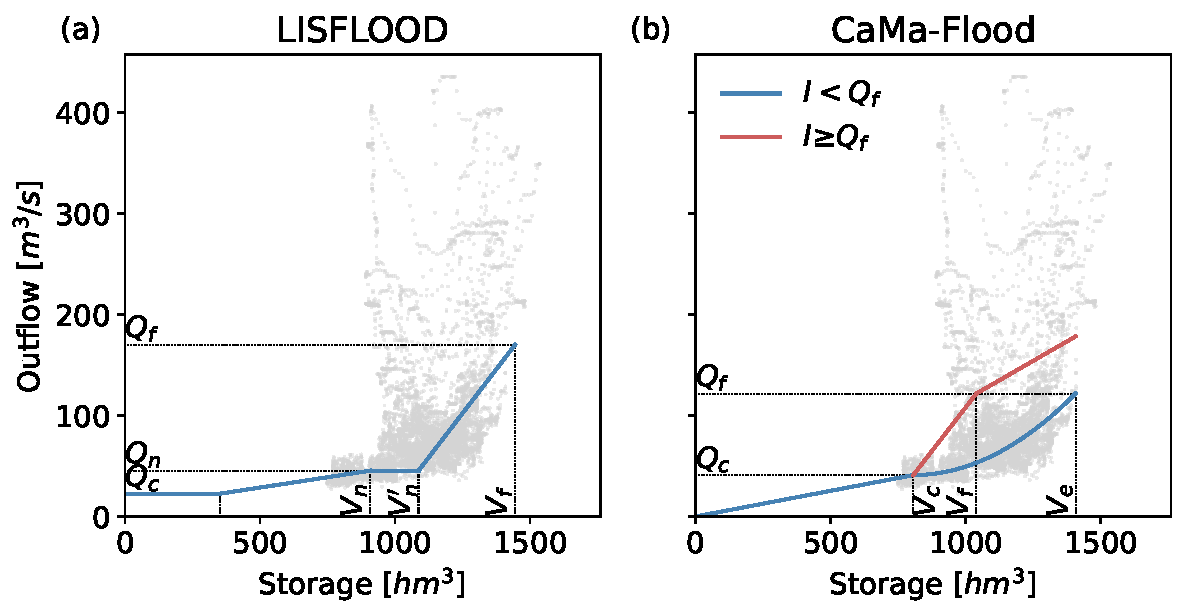
\includegraphics[width=\columnwidth]{figures/fig03.pdf}
    \caption{Storage–outflow relationships for the (a) LISFLOOD and (b) CaMa-Flood reservoir routines. The curves illustrate the calibrated operational rules for the Yellowtail dam (GRanD ID 355). Grey points represent observed daily records, highlighting the spread of historical operations.}
    \label{fig:lisflood_camaflood}
\end{figure}

\subsubsection{CaMa-Flood}
\label{sec:camaflood}

The reservoir module in the Catchment-based Macro-scale Floodplain model (CaMa-Flood) \citep{Hanazaki2022} represents an evolution of the LISFLOOD approach by introducing inflow-dependency into the operational logic. Unlike the static LISFLOOD scheme, CaMa-Flood distinguishes between two operational modes based on the current inflow ($I_t$).

When $I_t$ is below a threshold ($Q_f$), the outflow is modeled as a quadratic function of storage. This non-linear behavior restricts releases as the reservoir empties, effectively conserving water for future demand. Conversely, when $I_t$ exceeds $Q_f$, the system transitions toward a linear reservoir behavior to manage high-flow conditions. 

\begin{equation}
\label{eq:camaflood}
    \begin{aligned}
    & Q_t = \\
    & \begin{cases}
        \begin{cases}
            Q_n \frac{V_t}{V_f} & \qquad \qquad \qquad \quad \;  V_t < V_c \\
        \end{cases} & \forall \, I_t \\[2ex]
        \begin{cases}
            Q_c + \bigl( \frac{V_t - V_c}{V_e - V_c} \bigr)^2 \Delta Q & \quad \;\;\;\, V_c \leq V_t < V_e \\
            Q_f & \quad \;\;\;\, V_t \geq V_e
        \end{cases} & I_t < Q_f \\[2ex]
        \begin{cases} 
            Q_c + \frac{V_t - V_c}{V_f - V_c} \Delta Q & V_c \leq V_t < V_f \\
            Q_f + k \frac{V_t - V_f}{V_e - V_f} (I_t - Q_f) & V_f \leq V_t < V_e \\
            I_t & V_t \geq V_e
        \end{cases} & I_t \geq Q_f
    \end{cases} \\[1ex]
    & \text{where } Q_c = Q_n \frac{V_c}{V_f} \text{ and } \Delta Q = Q_f - Q_c
    \end{aligned}
\end{equation}

where $V_e$ is the emergency storage limit—defined as the upper part of the flood zone— and $k$ is the release coefficient that regulates outflows under flood conditions based on available storage capacity. \citet{Hanazaki2022} defined $k$ as a fixed value derived from the total flood volume (Eq.~\ref{eq:hanazaki_k}). Under that formulation, $k$ becomes zero for high-regulation reservoirs, resulting in a constant release even as storage levels approach $V_e$, effectively neglecting the exhaustion of regulation capacity. To address this unrealistic behavior, we introduced a dynamic calculation of $k$ at each time step based on the instantaneous reservoir volume ($V_t$, Eq.~\ref{eq:new_k}). This modification ensures that $k$ increases as storage approaches $V_e$, facilitating higher discharge to mitigate the risk of overtopping.

\begin{subequations}
    \label{eq:camaflood_release_coefficient}
    \begin{align}
        k &= \max \Bigl( 1 - \frac{V_{\max} - V_f}{A_{c} \cdot 0.2}, 0 \Bigr) \label{eq:hanazaki_k}\\
        k &= \max \Bigl( 1 - \frac{V_{\max} - V_t}{A_{c} \cdot 0.2}, 0 \Bigr) \label{eq:new_k}
    \end{align}
\end{subequations}

While \citet{Hanazaki2022} utilized default parameters, we calibrated five parameters (Table~\ref{tab:parameters_camaflood}) to ensure the routine has comparable degrees of freedom to the other routines. To maintain consistency with the LISFLOOD benchmark, three parameters ($\alpha$, $\delta$, $\epsilon$) share identical definition across both models.

\begin{table*}[t]
    \centering
    \begin{threeparttable}
        \caption{Calibration parameters in the CaMa-Flood reservoir module.}
        \label{tab:parameters_camaflood}
        \begin{tabularx}{\textwidth}{lXlclll}
            \toprule
            \textbf{Parameter} & \textbf{Description} & \textbf{Definition} & \textbf{Minimum} & \textbf{Maximum} & \textbf{Default} \\
            \midrule
            $\alpha$\tnote{*} & Fraction of the total storage corresponding to the flood limit & $V_f = \alpha V_{\max}$ & 0.2 & 0.99 & 0.97 \\
            $\beta$ & Proportion between flood limit and total storage corresponding to the extreme limit & $V_e = V_{\max} - \beta (V_{\max} - V_f)$ & 0.001 & 0.999 & 0.2 \\
            $\gamma$ & Proportion of the flood limit corresponding to the normal limit & $V_c = \gamma V_f$ & 0.001 & 0.999 & 0.5 \\
            $\delta$\tnote{*} & Factor of the 100-year inflow ($I_{100}$) that defines the flood outflow & $Q_f = \delta I_{100}$ & 0.1 & 0.5 & 0.3 \\
            $\epsilon$\tnote{*} & Ratio between normal and flood outflows & $Q_n = \epsilon Q_f$ & 0.001 & 0.999 & $Q_f / \bar{I}$ \\
             \bottomrule
        \end{tabularx}
        \begin{tablenotes}
            \small
            \item{*} Parameter identical in LISFLOOD and CaMa-Flood.
        \end{tablenotes}
    \end{threeparttable}
\end{table*}

The primary advantage of the CaMa-Flood routine over LISFLOOD is its ability to represent a non-unique relationship between storage and outflow (Fig.~\ref{fig:lisflood_camaflood}). By incorporating $I_t$ into the operational rules, the routine can better capture the observed dispersion in the storage-outflow values, providing a more realistic representation of human-regulated flow variability.

\subsubsection{mHM}
\label{sec:mhm}

The reservoir module within the Multiscale Hydrological Model (mHM) \citep{Samaniego2010, Kumar2013, Thober2019} represents a fundamental shift in modeling philosophy compared to the LISFLOOD and CaMa-Flood routines. Rather than treating outflow as a direct function of storage, the mHM routine determines releases primarily based on a water demand time series ($D_t$). While \citet{Shrestha2024} utilized random forests to predict $D_t$ for individual reservoirs, we implement a seasonal approach to maintain model portability.

In our implementation, we derive an annual demand climatology by computing the mean observed outflow for each day of the year across the available records. To ensure this signal reflects demand rather than total outflow, we apply the water stress ($\bar{D} / \bar{I}$) as scaling factor, and smooth the signal using a 28-day moving average. This smoothed climatology serves as the seasonal demand signal $D_t$ for each reservoir, introducing the temporal variability missing in static storage–discharge schemes.

\medskip
\textbf{Reservoir release.} The total daily release $Q_t$ is partitioned into a component satisfying the hedged demand ($\hat{D}_t$) and a component representing the passthrough of inflow ($I_t$):

\begin{equation}
\label{eq:mhm}
    Q_t = \rho \cdot \kappa_t \cdot \hat{D}_t + (1 - \rho) \cdot I_t
\end{equation}

The partition coefficient $\rho$ is a function of the reservoir's degree of regulation ($\text{DOR}$). For highly regulated reservoirs ($\text{DOR} \geq \alpha$), the release is entirely demand-driven ($\rho = 1$). In all other cases, the influence of demand relative to inflow is governed by the parameters $\alpha$ and $\beta$:

\begin{equation}
\label{eq:partition_coeff}
    \rho = \min\left(1, \left( \frac{\text{DOR}}{\alpha} \right)^\beta \right)
\end{equation}

The demand component is further moderated by a time-varying coefficient $\kappa_t$, which hedges the release based on the current storage level $V_t$ relative to a target normal storage $V_n$:

\begin{equation}
\label{eq:mhm_kappa}
    \kappa_t = \Bigl( \frac{V_t}{V_n} \Bigr)^\lambda = \Bigl( \frac{V_t}{\gamma \cdot V_{\max}} \Bigr)^\lambda
\end{equation}
where $\gamma$ defines the normal storage fraction and $\lambda$ controls the sensitivity of the hedging to storage deficits.

\medskip
\textbf{Demand hedging.} The hedged demand $\hat{D}_t$ is calculated based on the ratio between average annual demand ($\overline{D}$) and inflow ($\overline{I}$). The parameter $\omega$ represents the expected annual water surplus and is used to categorize the reservoir's water stress. If there is no water stress ($\overline{D}/\overline{I} < 1 - \omega$), the daily demand ($D_t$) is supplied in addition to the average water surplus. If there is stress, the hedged demand is a combination of a fraction of the average inflow and a fraction of the daily demand.

\begin{equation}
\label{eq:hedged_demand}
    \hat{D}_t =
    \begin{cases}
        \overline{I} - \overline{D} + D_t  & \text{if } \frac{\overline{D}}{\overline{I}} < 1 - \omega \\
        \omega \cdot \overline{I} + (1 - \omega) \frac{\overline{I}}{\overline{D}} \cdot D_t & \text{otherwise}        
    \end{cases}
\end{equation}

\medskip
\textbf{Calibration.} Following the procedure established by \citet{Shrestha2024}, we calibrated five parameters (Table~\ref{tab:parameters_mhm}). Other authors used default values of some of the parameters \citep{Hanasaki2006, Shin2019, Sadki2023}, which we have used for the simulation with default parameters.

\begin{table*}[t]
    \centering
    \caption{Calibration parameters in the mHM reservoir module.}
    \begin{tabularx}{\textwidth}{lXllll}
        \toprule
       \textbf{Parameter} & \textbf{Description} & \textbf{Definition} & \textbf{Minimum} & \textbf{Maximum} & \textbf{Default} \\
        \midrule
        $\alpha$ & Threshold in the degree of regulation that defines demand-controlled reservoirs ($\text{DOR} > \alpha$) & Eq.~\ref{eq:partition_coeff} & 0.0 & 5.0 & 0.5 \\
        $\beta$ & It controls indirectly the proportion of inflow and demand in the releases & Eq.~\ref{eq:partition_coeff} & 0.5 & 3.0 & 1.0 \\
        $\gamma$ & Ration between normal and total storage & Eq.~\ref{eq:mhm_kappa} & 0.0 & 1.0 & 0.85 \\
        $\lambda$ & It further controls hedging based on the current reservoir storage & Eq.~\ref{eq:mhm_kappa} & 0.25 & 3.0 & 1.0 \\
        $\omega$ & It controls hedging based on the ratio between the current and average demand & Eq.~\ref{eq:hedged_demand} & 0.0 & 1.0 & 0.1 \\
         \bottomrule
    \end{tabularx}
    \label{tab:parameters_mhm}
\end{table*}

Unlike the rule-based schemes, the mHM routine produces a more realistic storage–outflow relationship, as the release is decoupled from the instantaneous storage volume and instead follows the seasonal cycle of demand. While more flexible, the main limitation of the routine is how to estimate the demand signals.

\subsubsection{STARFIT}
\label{sec:starfit}

The Storage Targets And Release Function Inference Tool (STARFIT) framework represents a data-driven paradigm that infers operational rules by learning the seasonality of reservoir storage and outflows \citep{Turner2021}. Unlike previous rule-based models, STARFIT employs harmonic functions to represent seasonal cycles. A key advantage of this formulation is its scale-independence; while the model parameters are typically fitted using weekly data to reduce noise, the harmonic frequency ($\omega$) can be adjusted for daily simulations ($\omega=1/365$), ensuring consistency with the temporal resolution of the simulation.

All variables are standardized to facilitate regionalization and comparison across basins (Eq.~\ref{eq:starfit_variables}). Storage is converted to reservoir filling, while inflow and outflow are expressed as normalized anomalies relative to the mean annual inflow ($\overline{I}$): 

\begin{subequations}
\label{eq:starfit_variables}
    \begin{align}
        \hat{V}_{t} &= \frac{V_t}{V_{\max}} \label{eq:standard_volume} \\
        \hat{Q}_{t} &= \frac{Q_t - \bar{I}}{\bar{I}} \label{eq:standard_outflow} \\
        \hat{I}_{t} &= \frac{I_t - \bar{I}}{\bar{I}} \label{eq:standard_inflow}
    \end{align}
\end{subequations}

\medskip
\textbf{Storage Normal Operating Range (NOR).} STARFIT defines the operational target of a reservoir through a Normal Operating Range (NOR), bounded by upper ($\text{NOR}_{\text{up}}$) and lower ($\text{NOR}_{\text{low}}$) seasonal harmonics. These bounds represent the typical filling levels for any given time of the year:

{\small
\begin{equation}
\label{eq:starfit_nor}
    \begin{alignedat}{2}
        \text{NOR}_{\text{up},t}   &= \min \Bigl( && \max \bigl( A + B \, \sin 2\pi\omega t + C \, \cos 2\pi\omega t, \; \hat{V}_{\min} \bigr), \\
                                   &              && \hat{V}_{\max} \Bigr) \\[1ex]
        \text{NOR}_{\text{low},t}  &= \min \Bigl( && \max \bigl( a + b \, \sin 2\pi\omega t + c \, \cos 2\pi\omega t, \; \hat{v}_{\min} \bigr), \\
                                   &              && \hat{v}_{\max} \Bigr) 
    \end{alignedat}
\end{equation}
}

where $t$ is the time (day or week) of the year. The NOR has 10 parameters: six defining the harmonic curves and four capping the maximum and minimum filling (Table~\ref{tab:parameters_starfit}). To fit these curves, the model uses only the three most extreme (highest and lowest) observed storage for each calendar week (Fig.~\ref{fig:starfit}), ensuring the NOR captures the envelope of historical operations.

\begin{figure}
    \centering
    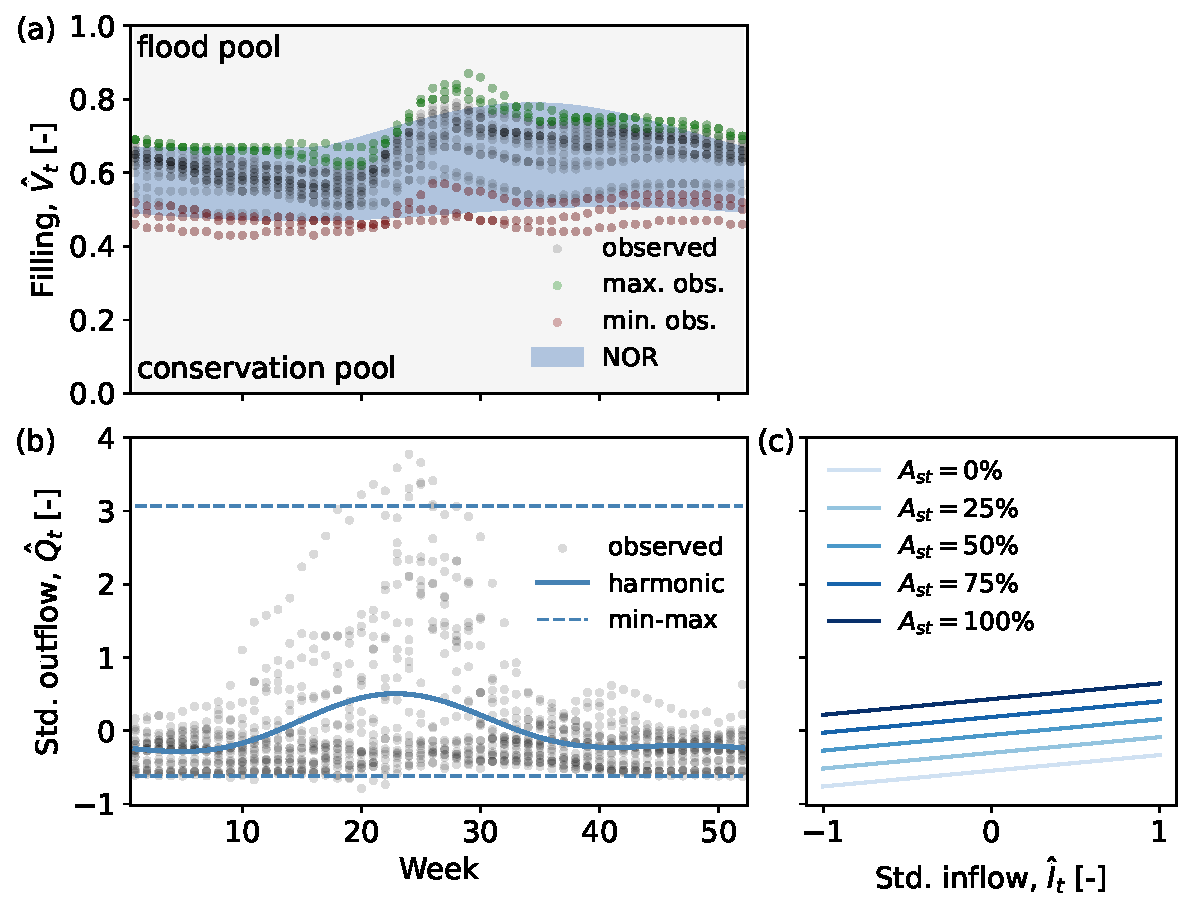
\includegraphics[width=\columnwidth]{figures/fig04.pdf}
    \caption{The STARFIT model for the Yellowtail dam (GRanD ID 355): (a) seasonal harmonic curves defining the storage normal operating range (NOR) for each calendar week; (b) the seasonal harmonic release; (c) the linear model of release residuals based on available storage ($A_{st}$) and standardized inflow.}
    \label{fig:starfit}
\end{figure}

\medskip
\textbf{Release function.} The release policy is conditioned on the reservoir's position relative to the NOR. To maintain the reservoir within its seasonal bounds, STARFIT applies a three-zone operational policy:

{\small
\begin{equation}
    \label{eq:starfit_release_harmonic}
    \begin{aligned}
    & Q_t = \\
    & \begin{cases}
        \min \Bigl( Q_{\min} + ( Q_{\text{NOR},t} - Q_{\min} ) \tfrac{\hat{V}_{t}}{\text{NOR}_{\text{low},t}}, I_t \Bigr) & \text{if } \hat{V}_{t} < \text{NOR}_{\text{low},t} \\[3ex]
        \max \Bigl( Q_{\min}, \, \min ( Q_{\text{NOR},t} , Q_{\max} ) \Bigr) & \text{if } \hat{V}_{t} \in \text{NOR}_t \\[2ex]
        %\text{mid} ( Q_c, Q_{\text{NOR},t}, Q_{\max} ) & \text{if } \text{NOR}_{\text{low},t} \leq \hat{V}_{t} \leq \text{NOR}_{\text{up},t} \\[2ex]
        Q_{\text{NOR},t} + ( Q_{\max} - Q_{\text{NOR},t} ) \tfrac{\hat{V}_{t} - \text{NOR}_{\text{up},t}}{1 - \text{NOR}_{\text{up},t}} & \text{if } \hat{V}_{t} > \text{NOR}_{\text{up},t}
    \end{cases}
    \end{aligned}
\end{equation}
}

We modified the definitions of the outflow for both below and above the NOR, as the original definitions produced in some cases noisy releases. In both cases, we have introduced a linear interpolation between a fixed minimum or maximum outflow ($Q_{\min}$ or $Q_{\max}$) and the outflow associated  with the respective NOR boundary ($Q_{\text{NOR}_{\text{low}},t}$ or $Q_{\text{NOR}_{\text{up}},t}$). Within the NOR, the standardized outflow ($\hat{Q}_{t}$) is modeled as the sum of an harmonic component ($\hat{Q}_{harm,t}$) and a linear component  ($\hat{Q}_{\text{lin},t}$) that accounts for the current storage and inflow:

{\small
\begin{equation}
\label{eq:starfit_release_linear}
    \begin{aligned}
        \hat{Q}_{\text{NOR},t} &= \hat{Q}_{\text{harm},t} + \hat{Q}_{\text{lin},t} \\[1ex]
        \hat{Q}_{\text{harm},t} &= d \, \sin 2\pi\omega t + e \, \cos 2\pi\omega t + f \, \sin 4\pi\omega t + g \, \cos 4\pi\omega t \\[1ex]
        \hat{Q}_{\text{lin},t} &= h + i \frac{\hat{V}_{t} - \text{NOR}_{\text{low},t}}{\text{NOR}_{\text{up},t} - \text{NOR}_{\text{low},t}} + j \cdot \hat{I}_{t}
    \end{aligned}
\end{equation}
}

The release harmonic allows for bimodal release patterns (e.g., two release peaks per year). The linear term is discarded if the linearity is weak ($R^2 < 0.2$), reverting to a purely seasonal policy.

The complete release model comprises 7 parameters (Table~\ref{tab:parameters_starfit}), fitted using the full historical record of weekly releases (Fig.~\ref{fig:starfit}). Additionally, the minimum and maximum releases ($Q_{\min}$ and $Q_{\max}$) are estimated as quantiles of the observed daily inflows; we have changed the original values of these quantiles to 1\% and 99\%, respectively.

\begin{table*}[t]
    \centering
    \begin{threeparttable}
        \caption{Parameters in the STARFIT reservoir module.}
        \label{tab:parameters_starfit}
        \begin{tabularx}{\textwidth}{llXl}
            \toprule
            \textbf{Variable} & \textbf{Parameter} & \textbf{Description} & \textbf{Definition} \\
            \midrule
            \textbf{Storage} & $A, a$\tnote{*} & Average filling & Eq.~\ref{eq:starfit_nor} \\
                             & $B, b$\tnote{*} & Coefficient of the sine component & Eq.~\ref{eq:starfit_nor} \\
                             & $C, c$\tnote{*} & Coefficient of the cosine component & Eq.~\ref{eq:starfit_nor} \\
                             & $\hat{V}_{\min}, \hat{v}_{\min}$\tnote{*} & Lower limit to the filling & Eq.~\ref{eq:starfit_nor} \\
                             & $\hat{V}_{\max}, \hat{v}_{\max}$\tnote{*} & Upper limit to the filling & Eq.~\ref{eq:starfit_nor} \\
            \midrule
            \textbf{Release} & $Q_{\min}$ & Minimum release & $Q_1$\tnote{**} \\
                             & $Q_{\max}$ & Maximum release & $Q_{99}$\tnote{**} \\
                             & $d$ & Coefficient of the sine component in the first release harmonic & Eq.~\ref{eq:starfit_release_linear} \\
                             & $e$ & Coefficient of the cosine component in the first release harmonic & Eq.~\ref{eq:starfit_release_linear} \\
                             & $f$ & Coefficient of the sine component in the second release harmonic & Eq.~\ref{eq:starfit_release_linear} \\
                             & $g$ & Coefficient of the cosine component in the second release harmonic & Eq.~\ref{eq:starfit_release_linear} \\
                             & $h$ & Intercept in the linear release & Eq.~\ref{eq:starfit_release_linear} \\
                             & $i$ & Coefficient of the linear release related to the current storage & Eq.~\ref{eq:starfit_release_linear} \\
                             & $j$ & Coefficient of the linear release related to the current inflow & Eq.~\ref{eq:starfit_release_linear} \\
             \bottomrule
        \end{tabularx}
        \begin{tablenotes}
            \small
            \item[*] Upper case refers to the upper NOR, and lower case to the lower NOR.
            \item[**] Percentiles of the observed daily flows.
        \end{tablenotes}
    \end{threeparttable}
\end{table*}

\subsection{Experimental design}
\label{sec:experimental_design}

To address our research questions, we conducted four distinct simulation experiments designed to evaluate the routines under varying levels of data availability and calibration complexity.

The first run evaluates model performance using default parameters sourced from the literature (see Tables~\ref{tab:parameters_lisflood}, \ref{tab:parameters_camaflood}, and~\ref{tab:parameters_mhm}). This experiment assesses the "out-of-the-box" reliability of the routines, which is particularly relevant for continental or global applications where historical operational data are unavailable.

The remaining three experiments involve local parameter optimization targeting different target variables:
\begin{itemize} 
    \item \calQ: Univariate calibration of reservoir outflow. This mirrors the standard calibration procedure for operational systems like EFAS/GloFAS, where model parameters are tuned to match observed streamflow. 
    \item \calV: Univariate calibration of reservoir storage. This experiment evaluates the potential for training routines using satellite-derived storage products, which is vital for ungauged basins. 
    \item \calQV: Bivariate calibration of both storage and outflow. This multi-objective approach analyzes the trade-offs in model fidelity and identifies the information loss associated with single-variable calibration. 
\end{itemize}

Parameter optimization was performed using the Shuffled Complex Evolution (SCEUA) algorithm \citep{Duan1993, Duan1994}, implemented via the \textit{Spotpy} Python library \citep{Houska2015}. For each reservoir, the algorithm was executed for up to 1,000 iterations using four complexes. Following the recommendations of \citet{Shen2024} for large-sample hydrology, we used the full length of the available daily time series for calibration to capture the widest possible range of hydrological conditions.

Performance was quantified using the modified Kling-Gupta Efficiency (\KGEmod) \citep{kling2012}, which decomposes performance into correlation, bias, and variability components. For the bivariate experiment, we integrated the individual \KGEmod\ scores into a single multi-objective metric:

{\small
\begin{subequations}
    \label{eq:metrics}
    \begin{align}
        &\text{KGE}' = 1 - \sqrt{(\alpha - 1)^2+ (\beta - 1)^2 + (\rho - 1)^2 } \label{eq:kge} \\
        &\text{KGE}'_{\text{bivariate}} = 1 - \sqrt{(1 - \text{KGE}'_Q)^2 + (1 - \text{KGE}'_V)^2} \label{eq:kge_bivariate}
    \end{align}
\end{subequations}
}
where $\rho$ is the Pearson correlation coefficient, $\alpha$ represents variability (ratio of coefficients of variation), and $\beta$ is the bias (ratio of means), defined as:
{\small
\begin{align}
    &\beta = \frac{\mu_{\text{sim}}}{\mu_{\text{obs}}} \label{eq:kge_beta} \\
    &\alpha = \frac{\text{CV}_{\text{sim}}}{\text{CV}_{\text{obs}}} \label{eq:kge_alpha}
\end{align}
}

While the LISFLOOD, CaMa-Flood, and mHM routines are optimized using the iterative SCEUA algorithm, STARFIT employs a direct statistical fitting procedure. This approach does not require a heuristic search. Instead, the storage model parameters are estimated in a two-step process: an initial ordinary least squares (OLS) regression provides a first guess for the three harmonic parameters, followed by a non-linear optimization using the L-BFGS-B algorithm to finalize all five parameters, including the upper and lower capping values ($\hat{V}_{\max}, \hat{V}_{\min}$). In contrast, the parameters for the release model are derived exclusively through OLS regression.

Because the original STARFIT formulation inherently requires observations of both storage (to define the NOR) and outflow (to define the release policy), it is only evaluated within the \calQV\ bivariate experiment. This ensures a consistent comparison between the statistically-derived STARFIT policies and the calibrated rule-based routines.

\section{Results}
\label{sec:results}

\subsection{Which target variable is most relevant for reservoir calibration?}
\label{sec:compare_variables}

Figure~\ref{fig:compare_variables} illustrates the performance of the three rule-based reservoir routines (LISFLOOD, CaMa-Flood, and mHM) across the four experimental configurations. The results highlight a critical dependency between the calibration objective and the model's ability to represent the dual states of discharge and storage.

\begin{figure*}
    \centering
    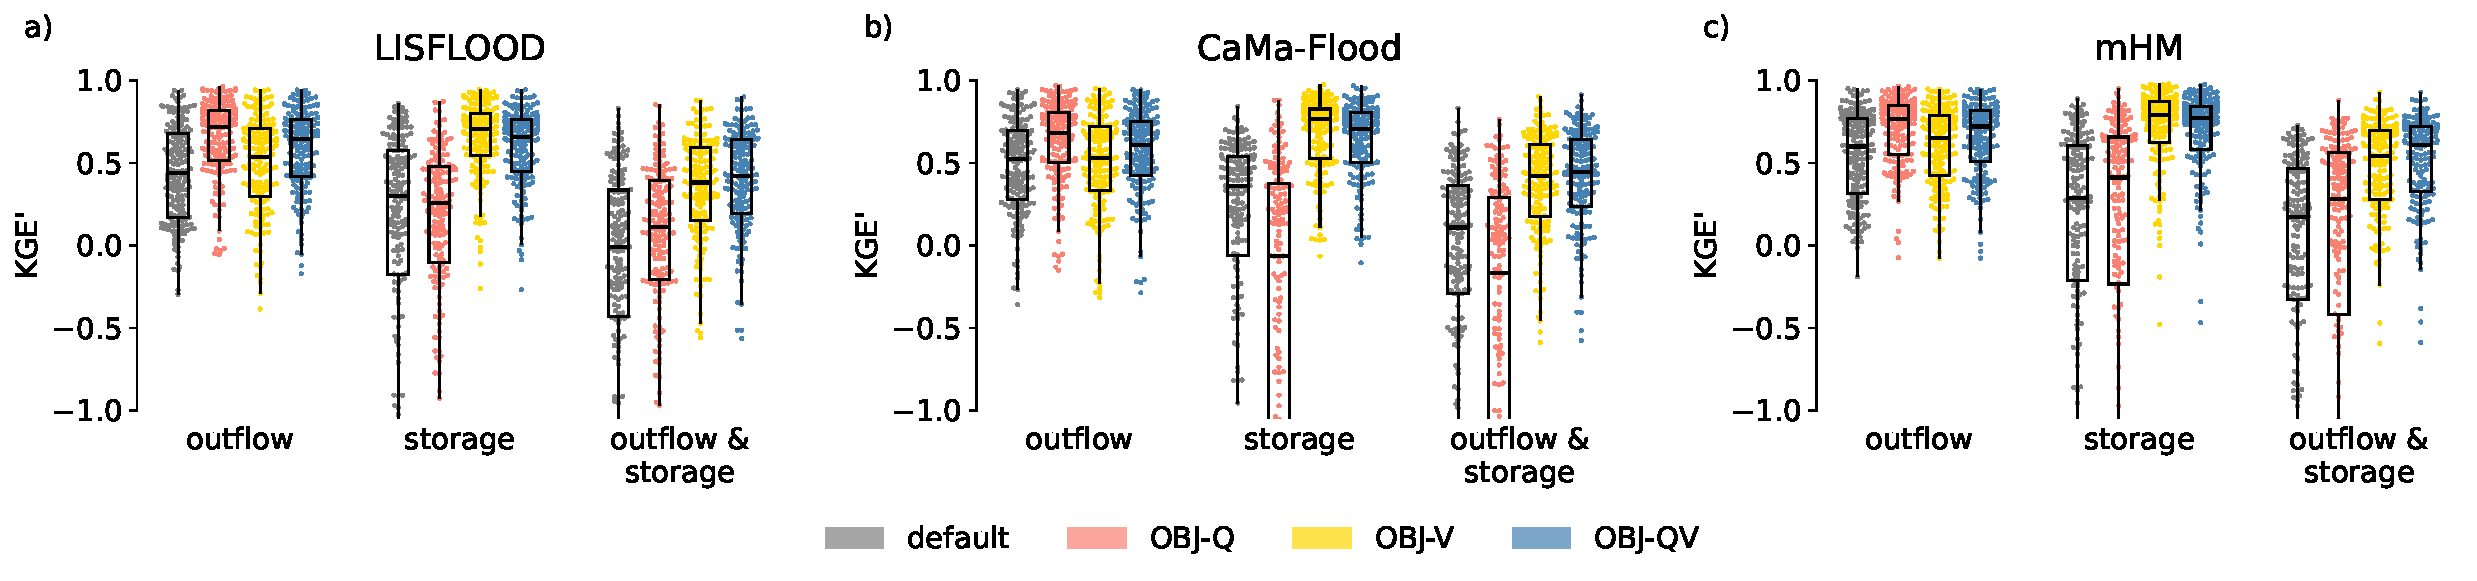
\includegraphics[width=1.0\textwidth]{figures/fig05.pdf}
    \caption{Comparison of the model performance depending on the variable(s) targeted in  the calibration. The panels correspond to the three reservoirs routines that were calibrated: a) LISFLOOD, b) CaMa-Flood and c) mHM. Within each panel, three groups of box plots show the performance in terms of outflow, storage, and both variables together. Four parameter sets are compared —default parameters, calibration of outflow (\calQ), storage (\calV) and both variables (\calQV)— indicated by colors. The dots represent individual reservoirs, indicating the distribution of the overall performance.}
    \label{fig:compare_variables}
\end{figure*}

The default parameterization (gray) provides a reasonably effective baseline for reservoir outflow across all three routines, with median \KGEmod\ values of 0.44, 0.52, and 0.60 for LISFLOOD, CaMa-Flood, and mHM, respectively. However, these default parameters fail to capture storage dynamics effectively; median \KGEmod\ scores for storage drop to 0.30, 0.36, and 0.29, respectively. The significantly larger interquartile range (IQR) in these scores indicates the high variability in storage performance across the 164 reservoirs. 

As expected, each routine achieves its peak performance for a specific variable when that variable is the sole target of the calibration. However, there is a clear trade-off when we look at how the models perform on variables they weren't trained on. Calibrating outflow (\calQ) severely degrades storage performance; in LISFLOOD and CaMa-Flood, this configuration yields the lowest median \KGEmod\ for storage among all experiments; in mHM, while the median is slightly higher than the default parameters, the dispersion between reservoirs is remarkably large. Conversely, calibrating to storage does not result in a similar degradation of outflow performance. In all three routines, \calV\ maintains outflow \KGEmod\ values that are superior to the default parameterization.

The bivariate calibration (\calQV) consistently achieves the highest combined performance across all routines. Notably, the performance of the \calQV\ run is closely mirrored by the storage-only calibration (\calV). These findings suggest that reservoir storage is a more informative variable than outflow for identifying model parameters.

While operational hydrology has traditionally relied on streamflow (outflow) for calibration, our results indicate that storage time series provide a more robust constraint on the internal state of the reservoir. This has significant implications for global hydrology, as it supports the feasibility of using satellite-derived storage products to calibrate reservoir routines in ungauged or data-poor regions \citep{Shen2025}.

\subsection{Which is the best-performing reservoir routine?}
\label{sec:compare_models}

Figure~\ref{fig:compare_models} compares the performance of the four routines across the different experimental configurations. Note that the outflow-only calibration (\calQ) is excluded here for simplicity, as the previous section demonstrated that it is a suboptimal strategy for capturing overall reservoir behavior.

\begin{figure*}
    \centering
    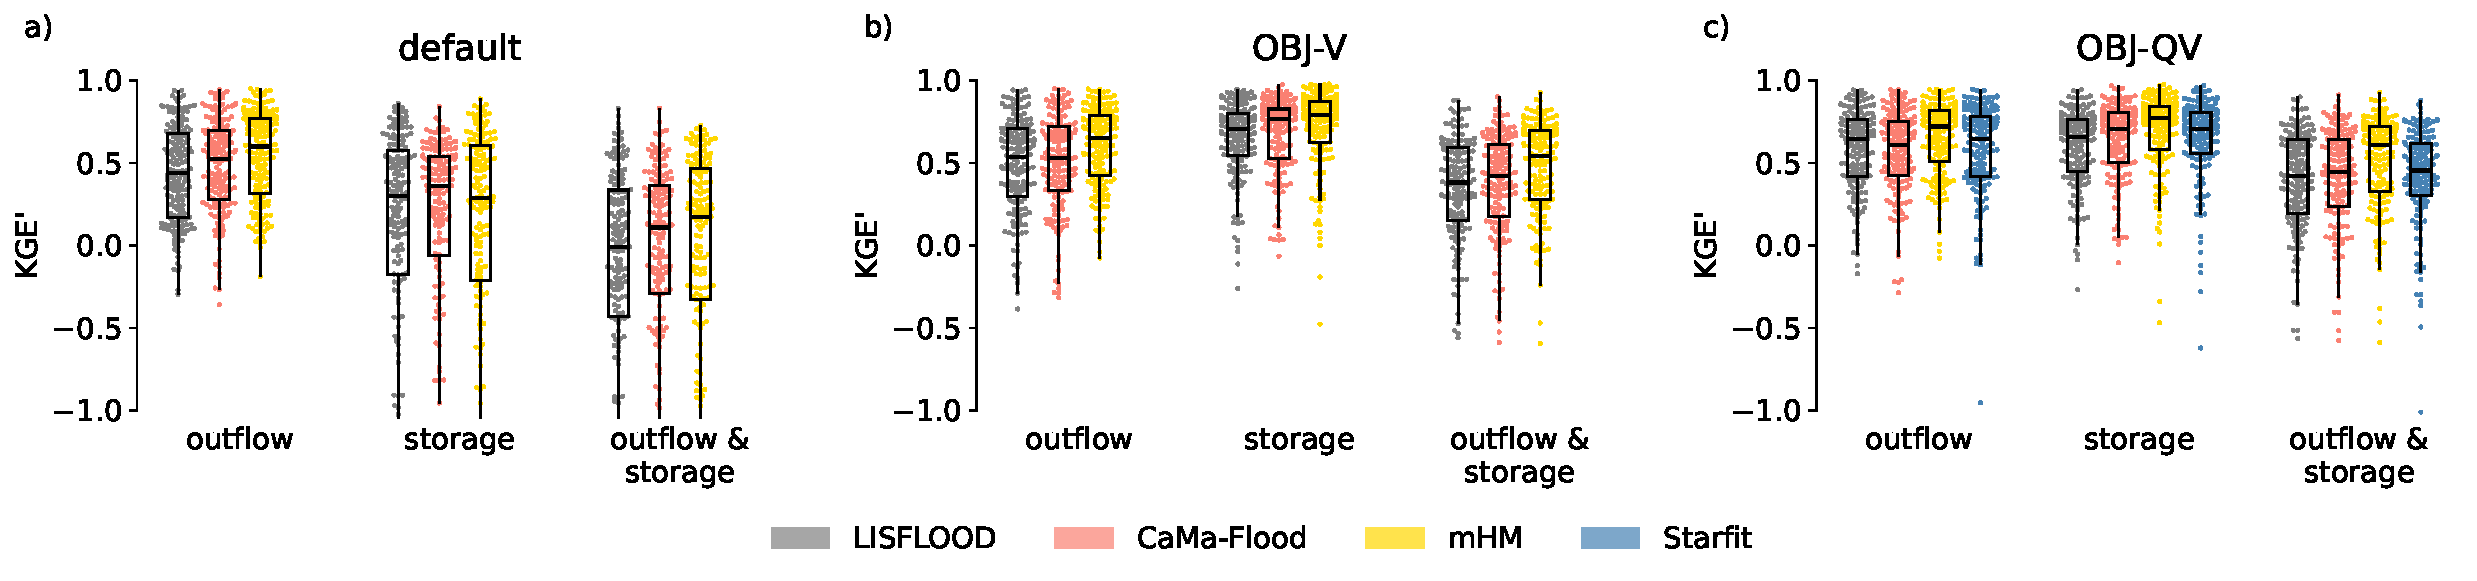
\includegraphics[width=1.0\textwidth]{figures/fig06.pdf}
    \caption{Comparison of the model performance depending on the reservoir routine. The panels correspond to three of the experiments: a) default parameters, b) calibration of storage (\calV), c) bivariate calibration of outflow and storage (\calQV). Within each panel, three groups of box plots show the performance in terms of outflow, storage, and both variables together. Four reservoir routines are compared— LISFLOOD, CaMa-Flood, mHM and STARFIT— indicated by colors. The dots represent individual reservoirs, indicating the distribution of overall performance.}
    \label{fig:compare_models}
\end{figure*}

Among the rule-based schemes, the mHM routine consistently achieves the highest performance across nearly all scenarios. Its primary strength lies in its ability to represent seasonal operations through demand-driven logic. The only exception is the uncalibrated (default) simulation of storage, where CaMa-Flood shows a slight advantage. Note that the CaMa-Flood routine was specifically designed for global applications without site-specific tuning \citep{Hanazaki2022}.

The results also highlight the benefits of model complexity: the CaMa-Flood routine, which evolved from the original LISFLOOD scheme by adding quadratic storage logic and inflow-dependency, systematically outperforms LISFLOOD in every experiment. This suggests that even small increases in the physical complexity of the storage-discharge relationship can significantly improve model performance.

Finally, the bivariate calibration results provide the first direct comparison with the STARFIT model. Despite its high parameterization (up to 19 parameters) and seasonal flexibility, STARFIT does not outperform mHM. Its combined performance is generally comparable to CaMa-Flood. This suggests that while seasonal harmonics are valuable, the structured rules in mHM and CaMa-Flood may provide a more robust framework for continuous daily simulations in large-scale hydrological models.

\DIFaddbegin \DIFadd{For a detailed analysis of model performance across each routine and variable, Appendix~\ref{app:kge_components} presents the decomposition of the \KGEmod.
}

\DIFaddend \subsection{How accurate is the reservoir shape approximation?}
\label{sec:reservoir_shape}

To represent the elevation–storage–area relationship in our modeling, we adopted a simplified geometric assumption where all reservoirs are treated as an inverted half-pyramid \citep{Liebe2005}. Under this assumption, the reservoir geometry is defined by the maximum surface area ($A_{\max}$) and the dam height ($H_{dam}$) (Eq.~\ref{eq:reservoir_geometry}). This approximation directly influences the calculation of the instantaneous surface area, which is a critical term for estimating direct precipitation and open-water evaporation.

While in situ observations of reservoir area are often unavailable, we validated this geometric assumption by comparing time series of estimated and observed water elevation. Time series of observed storage were converted into water elevations via Eq.~(\ref{eq:level}). These estimates were then compared against in situ observations for a subset of 138 reservoirs where such data were available. The performance of this elevation estimation is summarized in Fig.~\ref{fig:elevation_performance}.

\begin{figure*}
    \centering
    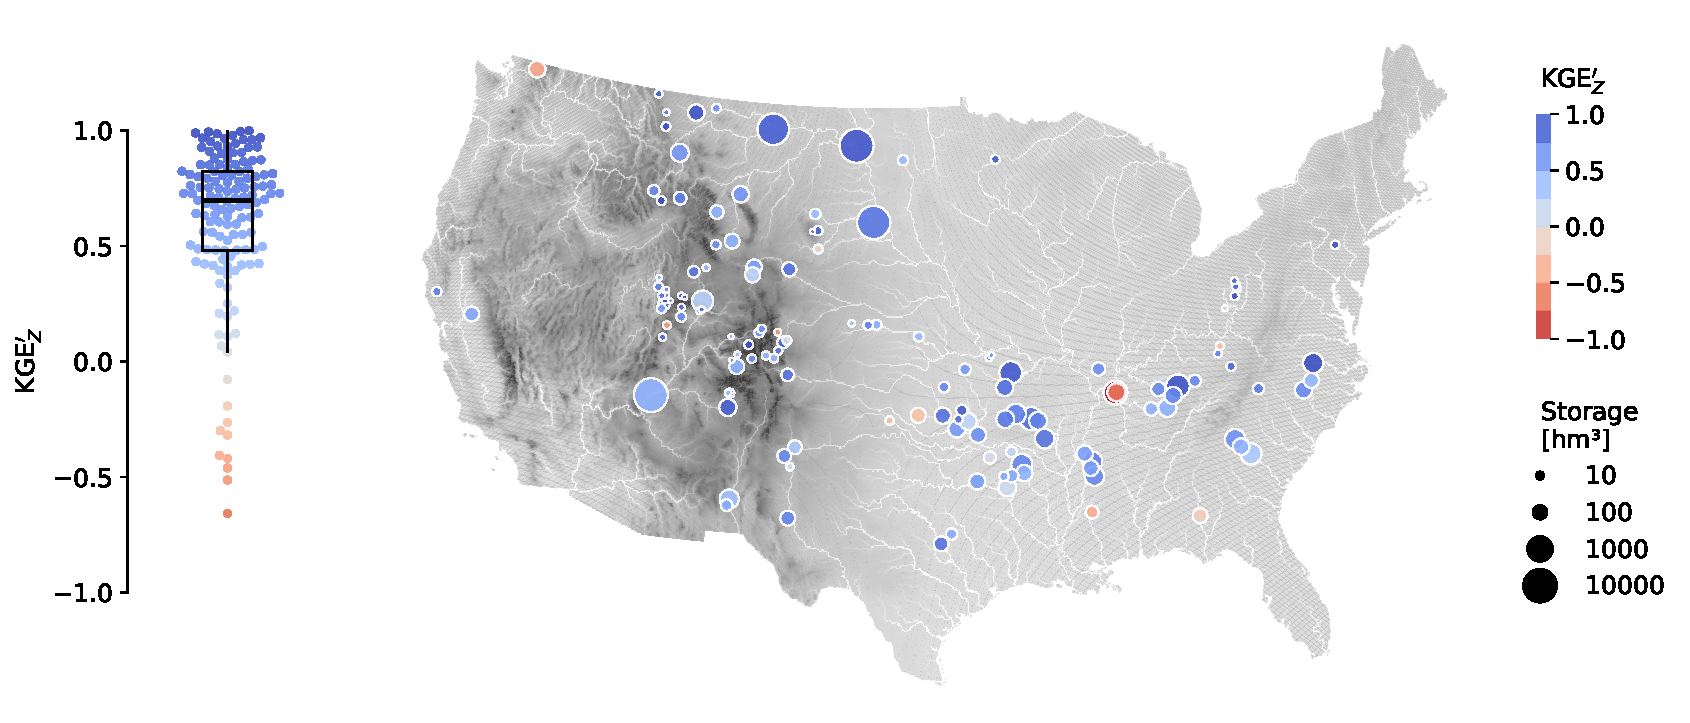
\includegraphics[width=1.0\textwidth]{figures/fig07.pdf}
    \caption{Performance of the reservoir level estimation assuming an inverted half-pyramid reservoir shape. The swarm plot on the left shows the overall distribution, where each point represents a reservoir and the box plot the quartiles. The map on the right shows the geographical distribution of performance; the dot size indicates storage capacity.}
    \label{fig:elevation_performance}
\end{figure*}

The inverted half-pyramid assumption proved to be a robust approximation for the majority of the study sites. The median \KGEmod\ for reservoir level estimation is 0.72, with 75\% of the reservoirs achieving a \KGEmod\ at least 0.44. From the three components of \KGEmod, the variability is the main cause of poor \DIFdelbegin \DIFdel{perfomance }\DIFdelend \DIFaddbegin \DIFadd{performance }\DIFaddend (median value of 1.25), whereas bias and correlation showed an overall good performance (median values of 1.00 in both cases). The accuracy of the level calculation is highly sensitive to the quality of the static attributes, specifically the crest elevation ($Z_{\max}$) and dam height ($H_{\text{dam}}$) (Eq.~\ref{eq:level}). As discussed in Section~\ref{sec:reservoir_attributes}, errors in global databases such as GRanD or GDW can propagate into these elevation estimates; therefore, data cleaning and the use of locally validated attributes are essential for accurate water-level modeling.



\section{Discussion}
\label{sec:discussion}

\subsection{Balancing model complexity and operational feasibility}
\label{sec:comparison_reservoirs}

This study compared reservoir routines of varying complexity, from the simple storage-dependent logic of LISFLOOD to the demand-driven and statistically-inferred policies of mHM and STARFIT. Our results indicate that model performance generally scales with the number of environmental covariates included in the routine (e.g., inflow or demand).

While mHM emerged as the best-performing routine (Section~\ref{sec:compare_models}), its dependence on a demand time series poses a significant operational challenge. In data-rich environments, demand can be inferred via machine learning \citep{Shrestha2024}, but in continental or global systems like EFAS or GloFAS, such data are often unavailable. 

A similar constraint applies to STARFIT, although its performance was not markedly superior to the more parsimonious CaMa-Flood routine. A distinct advantage of STARFIT for global applications is its flexibility across different temporal resolutions. The harmonic functions can be fitted at coarse or irregular temporal resolutions (such as those in satellite products) and be executed at daily resolution by adjusting the frequency term ($\omega$). For instance, \citet{Steyaert2025} recently demonstrated a global application of the STARFIT routine within the PCR-GLOBWB2 hydrological model by leveraging satellite-derived storage from the GloLAKES dataset \citep{Hou2024} to define the storage normal operating range (NOR). To explore this potential, Appendix~\ref{app:gww} provides a comparative analysis of the four reservoir routines when calibrated using satellite-derived storage estimates.

The CaMa-Flood routine has been selected for implementation in the forthcoming major evolution of the open-source LISFLOOD model (OS-LISFLOOD). This update will form the core of the upcoming EFAS~v6 and GloFAS~v5 operational systems \citep{Salamon2025}. These systems undergo regular updates encompassing updated meteorological forcing, revised surface fields, extended river discharge records and model developments. By evolving the reservoir logic to include inflow-dependency and quadratic storage--outflow relationships, we achieve a measurable gain in performance without increasing the data requirements for calibration. Furthermore, the robust default performance of the CaMa-Flood routine supports global applications in regions where historical records are sparse \citep{Hanazaki2022}.

\subsection{Current limitations and the forecast challenge}
\label{sec:limitations}

A notable limitation across the benchmarked routines is the absence of explicit reservoir purpose (e.g., irrigation, hydropower, or flood control...) \citep{Shen2025}. Reservoir operation is fundamentally driven by water demand, which varies significantly by use case. For instance, hydropower reservoirs are often maintained at high levels to maximize hydraulic head, whereas flood control reservoirs are drawn down ahead of wet seasons to maximize storage capacity. Conversely, irrigation reservoirs follow a distinct seasonal filling and release cycle to bridge the gap between wet-season supply and dry-season demand. 

While simple schemes like LISFLOOD or CaMa-Flood do not explicitly represent these operational rules, several studies have focused on purpose-specific modeling. This includes routines for water supply in the UK \citep{Salwey2024}, hydropower in France \citep{Baratgin2024}, and non-consumptive uses \citep{Shrestha2024}. Other approaches differentiate between irrigation and non-irrigation schemes \citep{Hanasaki2006, Sadki2023} or apply distinct objective functions based on the reservoir's primary use \citep{Haddeland2006}\DIFaddbegin \DIFadd{. Although the reservoir routines evaluated in this study do not explicitly consider reservoir purpose, Appendix~\ref{app:performance_use} shows the model performance disaggregated by the main reservoir use reported in GRanD}\DIFaddend .

In our comparison, the superior performance of mHM and STARFIT likely stems from their ability to capture these dynamics indirectly. mHM is a demand-driven routine that can infer specific usage patterns directly from demand time series, while STARFIT leverages observed seasonal patterns to learn operational behaviors. The fact that these two models outperformed LISFLOOD and CaMa-Flood, even if by a small margin, suggests that accounting for the temporal variability of human-driven demand is critical for improving global reservoir modeling.

Furthermore, these routines lack a forward-looking component, whereas in practice, reservoir operators rely on meteorological and hydrological forecasts across multiple timescales. While replacing current inflow with forecasted values could address this, it introduces a significant bottleneck for computationally demanding systems. The model would need to simulate the entire upstream catchment for the full forecast horizon before the reservoir release can be determined at any given node. While local or regional systems running simpler lumped models could potentially process these computations sequentially at each reservoir location, this remains a substantial implementation challenge for continental or global distributed systems.

\subsection{The potential of satellite products}
\label{sec:satellite_products}

The scarcity of in situ records remains the primary hurdle for large-scale reservoir modeling \citep{Shen2025}. Satellite-derived products offering reservoir area, elevation, and storage anomalies provide an opportunity to bridge this gap \citep{Zhao2018, Schwatke2020, Donchyts2022, Khandelwal2022, Hao2024, Hou2024}. Two of the outcomes of this study specifically support the transition toward using satellite products. First, we found that reservoir storage is a more informative calibration target than reservoir outflow, as storage-based calibration yields models that perform well across both state variables (Section~\ref{sec:compare_variables}). This represents a "lucky coincidence" for the community, as many available satellite products provide direct estimates of reservoir storage or storage variations rather than discharge. Second, our validation of the inverted half-pyramid shape (Section~\ref{sec:reservoir_shape}) suggests that even simplified geometric assumptions are sufficient to translate satellite-derived levels into volumes with reasonable accuracy. However, a rigorous analysis of the feasibility of remotely sensed data should consider also spatial and temporal resolution, apart from accuracy.

Recent studies are already leveraging these synergies; for instance, \citet{Shen2025} estimated monthly target storage values for 1,178 GRanD reservoirs by combining area time series from Global Water Watch (GWW) \citep{Donchyts2022} with area-storage curves from GRDL \citep{Hao2024}. This monthly target storage was integrated into an evolved reservoir scheme—based on LISFLOOD and CaMa-Flood—to introduce seasonality into otherwise simple storage--outflow formulations. 

The flexibility of STARFIT’s harmonic formulation is particularly well-suited for satellite data, as emphasized by \citet{Steyaert2025}. Because the frequency term in the harmonic curves allows the model to be fitted at coarser temporal resolutions (e.g., monthly satellite passes) and then run at a daily time step, it overcomes the temporal sampling limitations of many satellite products.

In line with \citet{Shen2025}, we have conducted a preliminary analysis of the potential use of the (GWW) dataset \citep{Donchyts2022}, as detailed in Appendix~\ref{app:gww}. Our findings indicate that while satellite-derived storage follows observed historical trends, a persistent bias often exists between in situ and remotely-sensed values. The primary bottleneck for the quality of these products is the availability of accurate elevation-storage-area curves. While several efforts have attempted to provide these curves globally \citep{Yigzaw2018, Busker2019, Khazaei2022}, they frequently show shortcomings when validated against in situ data.

\subsection{Toward data-driven reservoir modeling}
\label{sec:data-driven}

The recent revolution in deep learning has demonstrated that data-driven models can outperform traditional physical models in streamflow prediction \citep{Nearing2024}. To support a similar transition in reservoir modeling, we have formatted the ResOpsUS+CARS dataset following the CARAVAN standard \citep{Kratzert2023}. This extension of the original ResOpsUS dataset \citep{Steyaert2022} integrates the reservoir operations with meteorological time series, the reservoir attributes from GRanD/GDW, catchment characteristics from GloFAS static maps, and climate indices from ERA5. By consolidating these diverse covariates—encompassing reservoir morphology, catchment physiography, seasonality, meteorology and climate—we provide the necessary information for deep learning models to identify the complex drivers of reservoir release.  

Reservoir operations are the product of complex human-natural interactions that process-based routines struggle to capture entirely. While we acknowledge that deep learning offers a path toward superior performance, these models are notoriously data-hungry. This highlights the ongoing necessity of curated, multi-national observational datasets—not just for training, but for the rigorous benchmarking of the hybrid physical-statistical models and the development of global remotely-sensed approaches.


\section{Conclusions}
\label{sec:conclusions}

This study provided a comprehensive benchmarking of four reservoir routines (LISFLOOD, CaMa-Flood, mHM, and STARFIT) evaluated across 164 reservoirs in the United States using the ResOpsUS and GRanD datasets. By comparing different calibration strategies and model structures, we draw the following conclusions.

Reservoir storage is the most informative variable for calibration. Our results demonstrate a significant asymmetry in model identifiability. While calibrating routines to match observed outflow (the standard practice in many hydrological models) leads to a poor representation of internal reservoir states, calibrating to observed storage yields robust performance for both storage and outflow. This finding supports the shift toward using satellite-derived storage products for model parameterization, particularly in ungauged basins.

mHM offers superior performance, but CaMa-Flood provides the best operational balance. While the demand-driven logic of the mHM routine consistently demonstrated superior performance, its reliance on site-specific demand data constrains its applicability in continental and global systems where such information is often scarce. The CaMa-Flood routine, which will be integrated into the OS-LISFLOOD model, represents an optimal compromise: it provides significant improvements over the original linear storage logic without requiring additional input variables or data-intensive calibration.

The inverted half-pyramid geometric assumption is a robust approximation. Validating reservoir level estimations against in situ observations confirmed that a simplified inverted half-pyramid shape is sufficient for large-scale modeling. This validates the use of maximum area and dam height as sufficient proxies to link storage, area, and elevation, which is critical for estimating evaporative losses and integrating altimetry or reservoir area data.

STARFIT’s flexibility is a key asset for remote sensing integration. Although STARFIT did not outperform the rule-based mHM or CaMa-Flood routines in daily simulations, its harmonic formulation is uniquely capable of bridging temporal gaps in observations. Its ability to be fitted at monthly scales and run at daily resolutions makes it a powerful tool for leveraging current and future satellite altimetry missions.

Looking forward, the integration of reservoir modeling into global hydrology must move beyond the "data-poor" paradigm. The creation of standardized, multi-national datasets like the ResOpsUS+CARS is a step toward this goal. By providing these data in the CARAVAN format, we aim to facilitate the development of hybrid models that combine the physical consistency of process-based routines with the predictive power of deep learning. Such advancements will be essential for improving the accuracy of operational flood and drought forecasting systems in an increasingly managed global water cycle.


\codedataavailability{All the code used to generate the reservoir dataset, implement the four reservoir schemes, and perform the model calibrations is available in the following GitHub repository: \url{https://github.com/casadoj/reservoirs-LSHM}. The benchmarking dataset generated for this study can be accessed via Zenodo at \url{https://doi.org/10.5281/zenodo.15978041}.}


\appendix

\section{Evaluation of GWW storage estimates}
\label{app:gww}

To assess the feasibility of using Global Water Watch (GWW) \citep{Donchyts2022} for future global-scale reservoir calibration, we evaluated the accuracy of its volume estimates against our observational sample. Although GWW provides reservoir area for nearly all reservoirs in our dataset, storage data were available for only 12 of them. Figure~\ref{fig:gww_storage_performance} illustrates the performance and geographical distribution of this subset, comparing the observed storage time series against GWW estimates.

\begin{figure*}
    \centering
    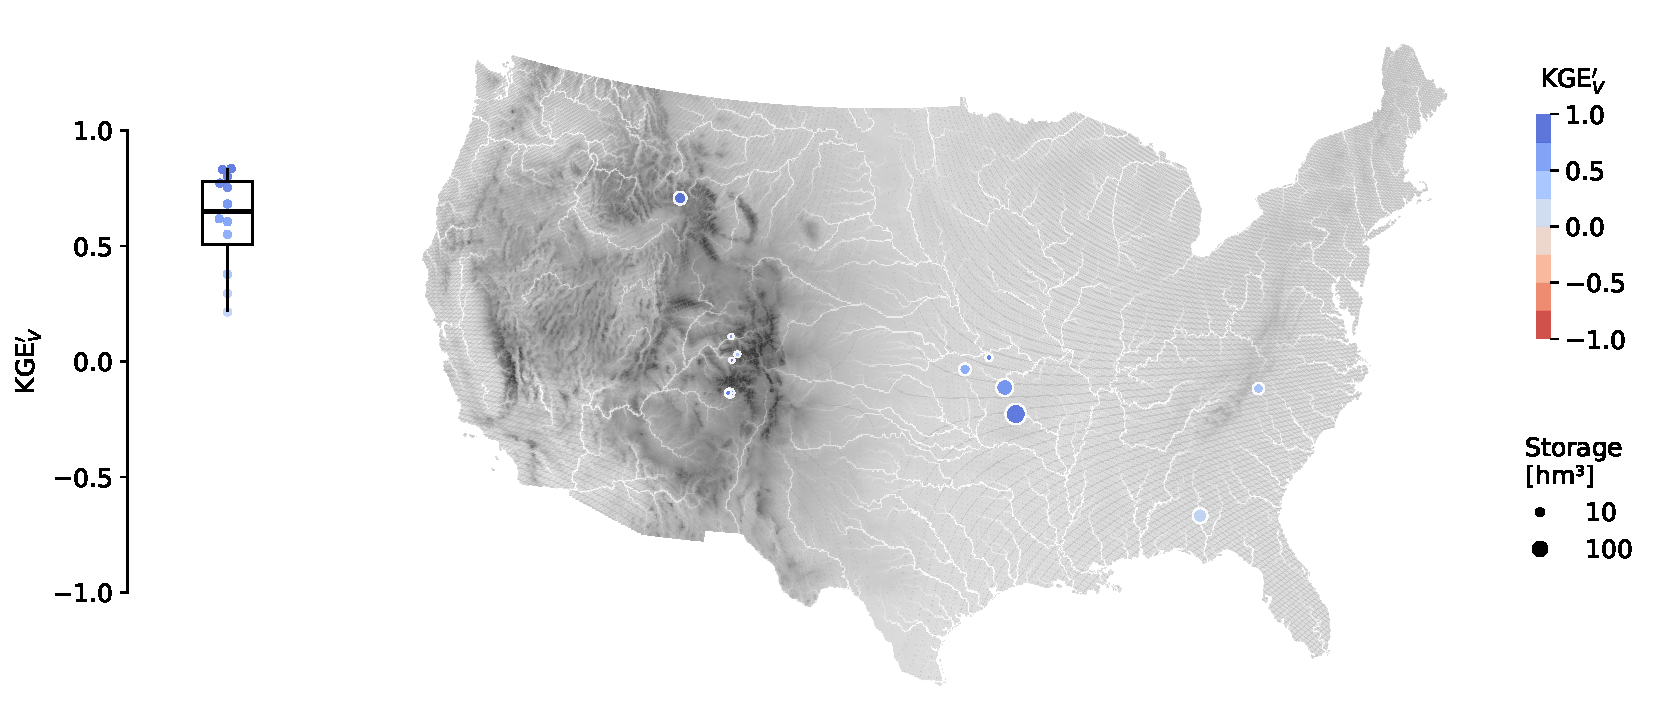
\includegraphics[width=1.0\textwidth]{figures/figA1.pdf}
    \caption{Performance of the reservoir storage estimates provided by the Global Water Watch. The swarm plot on the left shows the overall distribution, where each point represents a reservoir and the box plot the quartiles. The map on the right shows the geographical distribution of performance; the dot size indicates storage capacity.}
    \label{fig:gww_storage_performance}
\end{figure*}

Despite the limited sample size, GWW storage estimates demonstrate relatively high skill, with a median \KGEmod\ of 0.65 and 75\% of the reservoirs exceeding a score of 0.51. In terms of decomposition, GWW tends to overestimate total storage (median bias of 1.12 with an IQR of 0.13) while slightly underestimating variability (median of 0.91, IQR 0.37). Notably, the temporal dynamics are captured accurately, reflected by a median correlation of 0.88 (IQR 0.10).

To evaluate the feasibility of utilizing satellite products in future applications, we conducted a fifth experiment (\calGWW) wherein the reservoir schemes were calibrated against the storage estimates from GWW. This setup mirrors the univariate storage calibration experiment (\calV), with the distinct modification that the optimization target is a satellite-derived product rather than in situ observations. Because the STARFIT formulation requires both storage and outflow time series for its fitting procedure, this specific model was parameterized using observed outflow alongside the satellite-estimated storage. Figure~\ref{fig:gww_model_performance} illustrates the performance of this experiment validated against in situ observations (i.e., evaluated against the actual reservoir storage records rather than the satellite data used during optimization).

\begin{figure*}
    \centering
    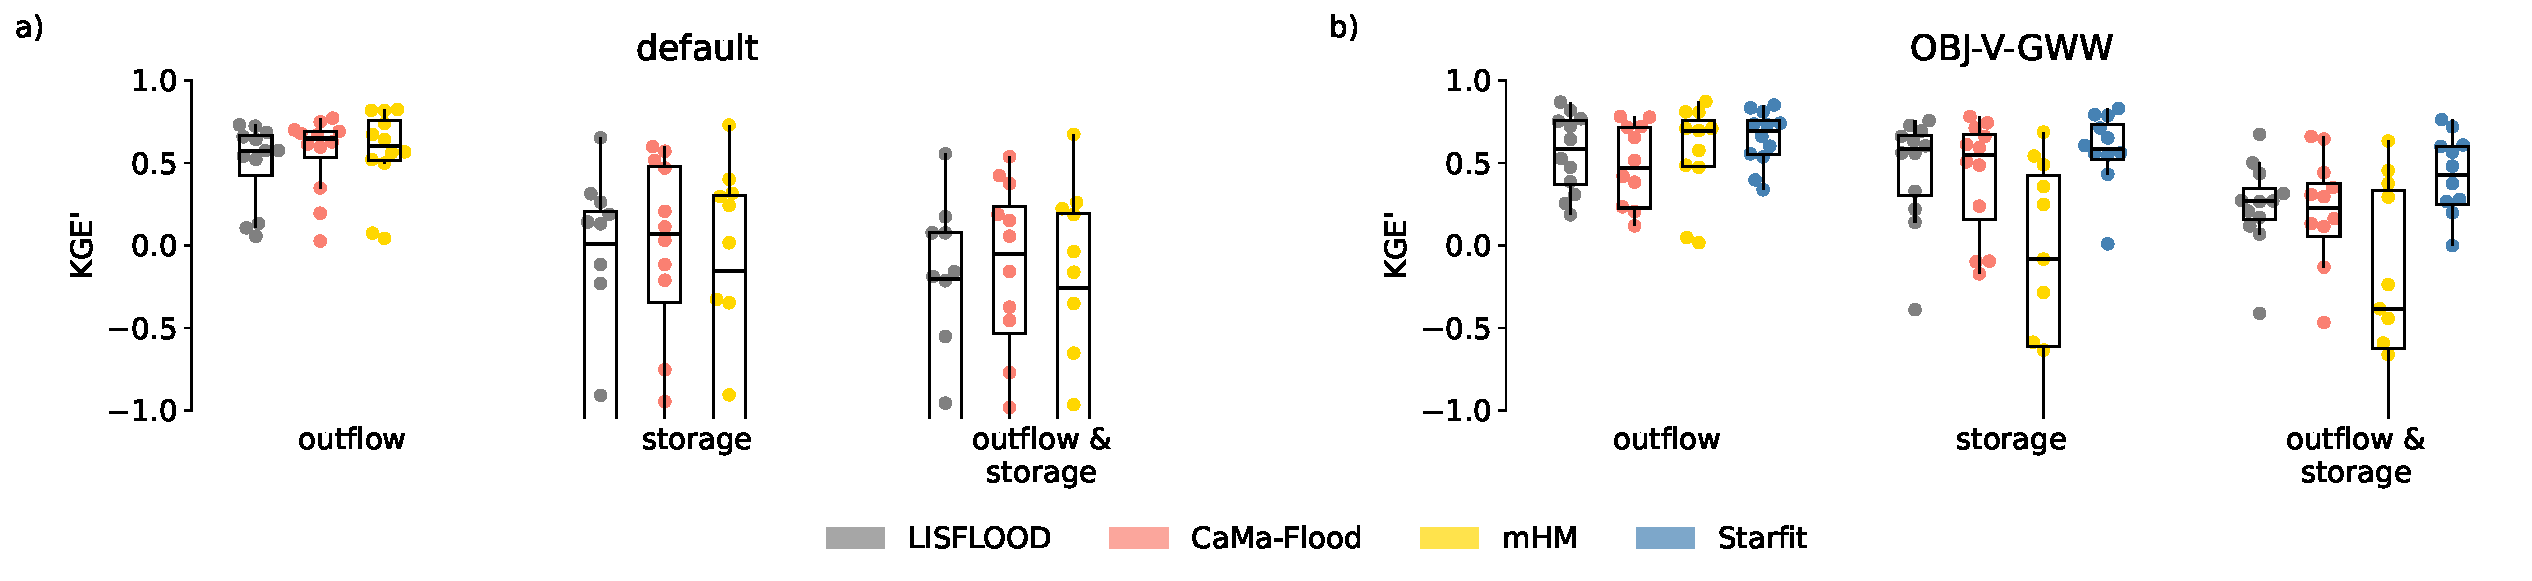
\includegraphics[width=1.0\textwidth]{figures/figA2.pdf}
    \caption{Comparison of model performance across different reservoir routines. The panels represent two experiments: a) default reservoir parameters, and b) univariate calibration using reservoir storage estimated by the Global Water Watch (\calGWW). Within each panel, three groups of box plots show the performance in terms of outflow, storage, and both variables combined. Four reservoir routines are compared— LISFLOOD, CaMa-Flood, mHM and STARFIT— indicated by colors. The dots represent individual reservoirs, indicating the distribution of overall performance.}
    \label{fig:gww_model_performance}
\end{figure*}

Calibration using the satellite product consistently yields performance improvements relative to the default parameter baselines. The LISFLOOD and CaMa-Flood routines appear to be particularly sensitive to the constraints of the satellite data. Both models experience a substantial surge in storage simulation performance, with median \KGEmod\ values increasing by 0.57 and 0.48 for LISFLOOD and CaMa-Flood, respectively. Interestingly, this enhancement does not impact outflow performance in LISFLOOD, whereas it noticeably degrades it in CaMa-Flood (a loss of 0.18 in median \KGEmod). 

Conversely, the satellite-based calibration yields negligible improvements for the mHM routine (gains of only 0.07 and 0.09 in median \KGEmod\ for storage and outflow, respectively), resulting in poor overall performance. This outcome contrasts sharply with the original \calV\ experiment, where univariate in situ storage calibration yielded good performance across all routines, including mHM.

While STARFIT emerges as the highest-performing routine in the \calGWW\ experiment, this comparison is inherently uneven. Because the fitting of this routine required a combination of satellite-estimated storage and observed in situ outflow, its setup is actually a bivariate calibration.

These findings must be interpreted with caution. The evaluation is constrained by a small sample size ($n = 12$) that features reservoirs where the default parameters perform poorly.

\section{Analysis of the \KGEmod\ components}
\label{app:kge_components}

Figure~\ref{fig:kge_components} shows the performance of the multiple simulation runs disaggregated into the individual \KGEmod\ components: variability ($\alpha$), bias ($\beta$), and correlation ($\rho$).
\begin{figure*}
    \centering
    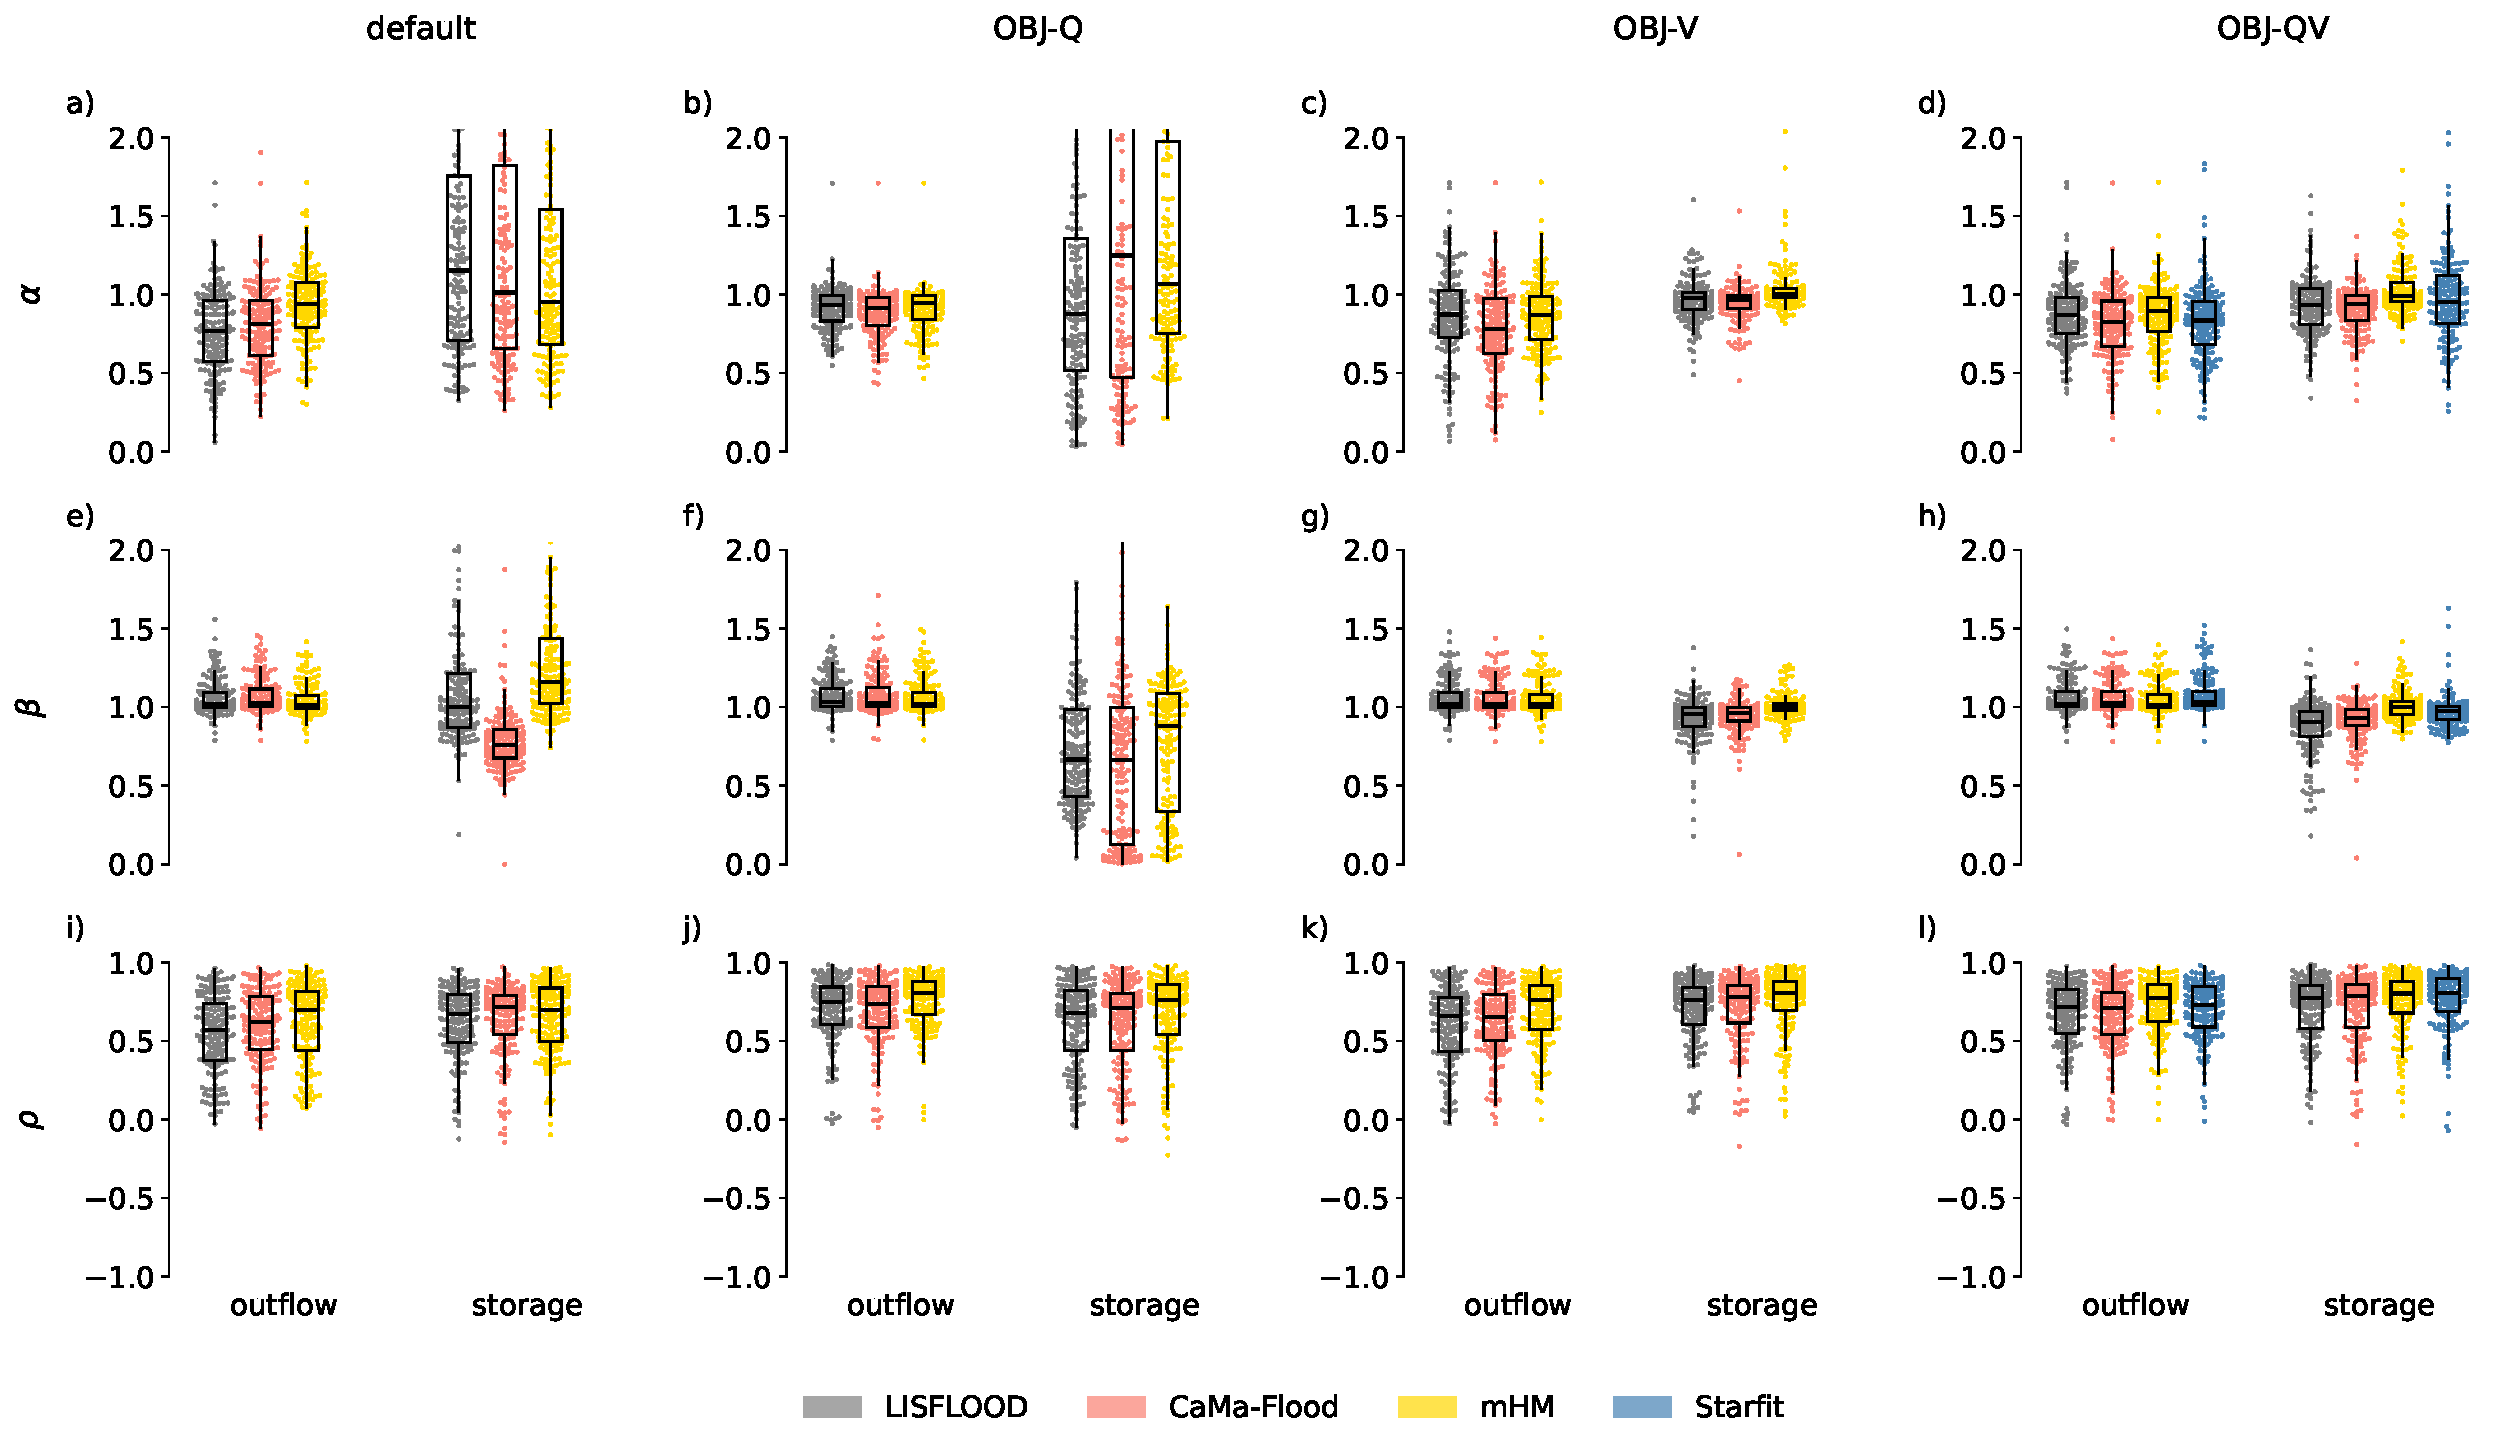
\includegraphics[width=1.0\textwidth]{figures/figB1.pdf}
    \caption{Comparison of the model performance in terms of variability ($\alpha$), bias ($\beta$) and correlation ($\rho$). The columns correspond to the four experiments: default parameters, calibration of outflow (\calQ), calibration of storage (\calV), and bivariate calibration of outflow and storage (\calQV). Within each panel, two groups of box plots show the performance in terms of outflow and storage. Four reservoir routines are compared— LISFLOOD, CaMa-Flood, mHM and STARFIT— indicated by colors. The dots represent individual reservoirs, indicating the distribution of overall performance.}
    \label{fig:kge_components}
\end{figure*}

The univariate calibration of outflow (\calQ) significantly degrades both the variability and bias of simulated storage. Conversely, the univariate calibration of storage (\calV) only marginally affects the correlation of simulated outflow and has a negligible impact on outflow variability and bias.

The superior performance of the mHM routine in the bivariate calibration (\calQV) is driven by its more accurate representation of outflow variability and correlation, as well as storage variability and bias.

\section{Performance by reservoir main use}
\label{app:performance_use}

The reservoir routines evaluated in this study are applied uniformly, regardless of the primary purpose of the reservoir. Table~\ref{tab:kge_use} analyses how the performance of these routines varies depending on the main reservoir use (as classified in the GRanD database). We exclusively present the values for the bivariate calibration, as it has been shown to yield the highest overall performance and provides the only equitable benchmark for the STARFIT model.

\begin{table*}[t]
    \centering
    \small
    \begin{tabular}{l rrrr @{\hspace{0.7cm}} rrrr @{\hspace{0.7cm}} r}
        \toprule
         \textbf{Main use}  & \multicolumn{4}{c}{\textbf{Storage}} & \multicolumn{4}{c}{\textbf{Outflow}} & \textbf{Count}\\
          & LISFLOOD & CaMa-Flood & mHM & STARFIT & LISFLOOD & CaMa-Flood & mHM & STARFIT & \\
         \midrule
        Flood control & 0.63 & \textbf{0.74} & 0.70 & 0.73 & 0.57 & 0.50 & \textbf{0.56} & 0.46 & 66 \\
        Hydropower    & 0.72 & 0.75 & \textbf{0.77} & 0.69 & 0.69 & 0.66 & \textbf{0.72} & 0.68 & 22 \\
        Irrigation    & 0.65 & 0.67 & \textbf{0.82} & 0.73 & 0.64 & 0.60 & \textbf{0.79} & 0.76 & 54 \\
        Navigation    & 0.24 & 0.28 & \textbf{0.35} & 0.33 & \textbf{0.87} & 0.86 & 0.86 & 0.84 & 4  \\
        Recreation    & 0.00 & 0.10 & -0.34 & \textbf{0.48} & 0.62 & 0.60 & \textbf{0.66} & 0.55 & 1  \\
        Water supply  & 0.55 & \textbf{0.74} & 0.73 & 0.56 & 0.67 & 0.65 & \textbf{0.71} & 0.60 & 17 \\
        \bottomrule
    \end{tabular}
    \caption{Model performance (in terms of median \KGEmod) in the bivariate calibration disaggregated by main reservoir use and reservoir routine. The table shows performance for both target variables: storage and outflow. Bold values indicate the best-performing routine for each reservoir use and target variable, and the \textit{Count} column indicates the number of reservoirs available in the dataset for that category.}
    \label{tab:kge_use}
\end{table*}

The mHM routine exhibits the highest performance across most categories. This superiority is particularly evident in the outflow simulations, where it is only outperformed by LISFLOOD in the Navigation category. Because mHM is a routine fundamentally driven by water demand time series, it follows logically that it captures release dynamics more effectively than routines primarily governed by available storage. Despite this structural orientation, mHM still emerges as the top-performing routine for storage simulations in three out of the six reservoir use categories. Meanwhile, CaMa-Flood reproduces storage variations slightly better in Flood Control and Water Supply reservoirs. Finally, we note that the lower apparent performance in the Navigation and Recreation categories is likely an artifact of their very small sample sizes.

\noappendix

%% Regarding figures and tables in appendices, the following two options are possible depending on your general handling of figures and tables in the manuscript environment:

%% Option 1: If you sorted all figures and tables into the sections of the text, please also sort the appendix figures and appendix tables into the respective appendix sections.
%% They will be correctly named automatically.

%% Option 2: If you put all figures after the reference list, please insert appendix tables and figures after the normal tables and figures.
%% To rename them correctly to A1, A2, etc., please add the following commands in front of them:

%\appendixfigures  %% needs to be added in front of appendix figures

%\appendixtables   %% needs to be added in front of appendix tables

%% Please add \clearpage between each table and/or figure. Further guidelines on figures and tables can be found below.



\authorcontribution{JCR designed the study, performed the data processing and analysis, and drafted the initial manuscript. JD assisted with data acquisition and processing and contributed to the manuscript revision. SG assisted in the experimental design and provided critical revisions of the results and the manuscript. PS conceptualized the study and supervised all stages of the research process.}

\competinginterests{The authors declare that they have no conflict of interest.} %% this section is mandatory even if you declare that no competing interests are present

%\disclaimer{TEXT} %% optional section

\begin{acknowledgements}
The authors would like to thank the creators and maintainers of the ResOpsUS, GRanD, and GDW datasets for making their data publicly available. We also acknowledge the use of ERA5 and GloFAS data provided by the European Commission's Copernicus Services.
The manuscript's style and LaTeX structure were refined with the assistance of the Gemini large language model (Google).
\end{acknowledgements}


%% REFERENCES

%% The reference list is compiled as follows:

% \begin{thebibliography}{}

% \bibitem[AUTHOR(YEAR)]{LABEL1}
% REFERENCE 1

% \bibitem[AUTHOR(YEAR)]{LABEL2}
% REFERENCE 2

% \end{thebibliography}

%% Since the Copernicus LaTeX package includes the BibTeX style file copernicus.bst,
%% authors experienced with BibTeX only have to include the following two lines:
%%
\bibliographystyle{copernicus}
\bibliography{bibliography.bib}
%%
%% URLs and DOIs can be entered in your BibTeX file as:
%%
%% URL = {http://www.xyz.org/~jones/idx_g.htm}
%% DOI = {10.5194/xyz}


%% LITERATURE CITATIONS
%%
%% command                        & example result
%% \citet{jones90}|               & Jones et al. (1990)
%% \citep{jones90}|               & (Jones et al., 1990)
%% \citep{jones90,jones93}|       & (Jones et al., 1990, 1993)
%% \citep[p.~32]{jones90}|        & (Jones et al., 1990, p.~32)
%% \citep[e.g.,][]{jones90}|      & (e.g., Jones et al., 1990)
%% \citep[e.g.,][p.~32]{jones90}| & (e.g., Jones et al., 1990, p.~32)
%% \citeauthor{jones90}|          & Jones et al.
%% \citeyear{jones90}|            & 1990



%% FIGURES

%% When figures and tables are placed at the end of the MS (article in one-column style), please add \clearpage
%% between bibliography and first table and/or figure as well as between each table and/or figure.

% The figure files should be labelled correctly with Arabic numerals (e.g. fig01.jpg, fig02.png).


%% ONE-COLUMN FIGURES

%%f
%\begin{figure}[t]
%\includegraphics[width=8.3cm]{FILE NAME}
%\caption{TEXT}
%\end{figure}
%
%%% TWO-COLUMN FIGURES
%
%%f
%\begin{figure*}[t]
%\includegraphics[width=12cm]{FILE NAME}
%\caption{TEXT}
%\end{figure*}
%
%
%%% TABLES
%%%
%%% The different columns must be seperated with a & command and should
%%% end with \\ to identify the column brake.
%
%%% ONE-COLUMN TABLE
%
%%t
%\begin{table}[t]
%\caption{TEXT}
%\begin{tabular}{column = lcr}
%\tophline
%
%\middlehline
%
%\bottomhline
%\end{tabular}
%\belowtable{} % Table Footnotes
%\end{table}
%
%%% TWO-COLUMN TABLE
%
%%t
%\begin{table*}[t]
%\caption{TEXT}
%\begin{tabular}{column = lcr}
%\tophline
%
%\middlehline
%
%\bottomhline
%\end{tabular}
%\belowtable{} % Table Footnotes
%\end{table*}
%
%%% LANDSCAPE TABLE
%
%%t
%\begin{sidewaystable*}[t]
%\caption{TEXT}
%\begin{tabular}{column = lcr}
%\tophline
%
%\middlehline
%
%\bottomhline
%\end{tabular}
%\belowtable{} % Table Footnotes
%\end{sidewaystable*}
%
%
%%% MATHEMATICAL EXPRESSIONS
%
%%% All papers typeset by Copernicus Publications follow the math typesetting regulations
%%% given by the IUPAC Green Book (IUPAC: Quantities, Units and Symbols in Physical Chemistry,
%%% 2nd Edn., Blackwell Science, available at: http://old.iupac.org/publications/books/gbook/green_book_2ed.pdf, 1993).
%%%
%%% Physical quantities/variables are typeset in italic font (t for time, T for Temperature)
%%% Indices which are not defined are typeset in italic font (x, y, z, a, b, c)
%%% Items/objects which are defined are typeset in roman font (Car A, Car B)
%%% Descriptions/specifications which are defined by itself are typeset in roman font (abs, rel, ref, tot, net, ice)
%%% Abbreviations from 2 letters are typeset in roman font (RH, LAI)
%%% Vectors are identified in bold italic font using \vec{x}
%%% Matrices are identified in bold roman font
%%% Multiplication signs are typeset using the LaTeX commands \times (for vector products, grids, and exponential notations) or \cdot
%%% The character * should not be applied as mutliplication sign
%
%
%%% EQUATIONS
%
%%% Single-row equation
%
%\begin{equation}
%
%\end{equation}
%
%%% Multiline equation
%
%\begin{align}
%& 3 + 5 = 8\\
%& 3 + 5 = 8\\
%& 3 + 5 = 8
%\end{align}
%
%
%%% MATRICES
%
%\begin{matrix}
%x & y & z\\
%x & y & z\\
%x & y & z\\
%\end{matrix}
%
%
%%% ALGORITHM
%
%\begin{algorithm}
%\caption{...}
%\label{a1}
%\begin{algorithmic}
%...
%\end{algorithmic}
%\end{algorithm}
%
%
%%% CHEMICAL FORMULAS AND REACTIONS
%
%%% For formulas embedded in the text, please use \chem{}
%
%%% The reaction environment creates labels including the letter R, i.e. (R1), (R2), etc.
%
%\begin{reaction}
%%% \rightarrow should be used for normal (one-way) chemical reactions
%%% \rightleftharpoons should be used for equilibria
%%% \leftrightarrow should be used for resonance structures
%\end{reaction}
%
%
%%% PHYSICAL UNITS
%%%
%%% Please use \unit{} and apply the exponential notation


\end{document}
